\documentclass[modern]{aastex61}

% All the packages
%\usepackage[letterpaper]{geometry}
\usepackage{fontspec}
\usepackage{microtype}
\usepackage{url}
\usepackage{amsmath}
\usepackage{mathtools}
\usepackage{esint}
\usepackage{amssymb}
\usepackage{natbib}
\usepackage{multirow}
\usepackage{graphicx}
\usepackage{scalerel}
\usepackage{calc}
\usepackage{etoolbox}
\usepackage{marginnote}
\usepackage{nicefrac}
\usepackage{tabstackengine}
\usepackage{diagbox}
\usepackage[makeroom]{cancel}
\usepackage{mathdots}
\usepackage{bbm}
\usepackage{booktabs}
\usepackage{xspace}
\usepackage{upgreek}
\usepackage[T1]{fontenc} % https://tex.stackexchange.com/a/166791
\usepackage{textcomp}
\usepackage{ifxetex}
\ifxetex
\usepackage{fontspec}
\defaultfontfeatures{Extension = .otf}
\fi
\usepackage{fontawesome}
\usepackage{listings}
\usepackage{mathtools}
\stackMath

% Page breaks in long equations
%\allowdisplaybreaks

% Bibliography stuff
\bibliographystyle{aasjournal}

% Shorthand for this paper
\newcommand{\starry}{\textsf{starry}\xspace}
\newcommand{\batman}{\textsf{batman}\xspace}
\newcommand{\planetplanet}{\textsf{planetplanet}\xspace}
\newcommand{\Python}{\textsf{Python}\xspace}
\newcommand{\cpp}{\textsf{C}++\xspace}
\newcommand{\Mathematica}{\textsf{Mathematica}\xspace}

% editing
\newcommand{\todo}[1]{{\color{red}\textbf{TODO:} #1}}


% References to text content
\newcommand{\documentname}{\textsl{article}}
\newcommand{\figureref}[1]{\ref{fig:#1}}
\newcommand{\Figure}[1]{Figure~\figureref{#1}}
\newcommand{\figurelabel}[1]{\label{fig:#1}}
\renewcommand{\eqref}[1]{\ref{eq:#1}}
\newcommand{\Eq}[1]{Equation~(\eqref{#1})}
\newcommand{\eq}[1]{\Eq{#1}}
\newcommand{\eqalt}[1]{Equation~\eqref{#1}}
\newcommand{\eqlabel}[1]{\label{eq:#1}}

% Add code, proof, and animation hyperlinks
\definecolor{linkcolor}{rgb}{0.1216,0.4667,0.7059}
\newcommand{\codeicon}{{\color{linkcolor}\faFileCodeO}}
\newcommand{\prooficon}{{\color{linkcolor}\faPencilSquareO}}
\newcommand{\animicon}{{\color{linkcolor}\faPlayCircle}}
\input{gitlinks}

\newtagform{eqtag}[]{(}{)}
\newcommand{\currentlabel}{None}

% Define a proof environment
\newenvironment{proof}[1]{%
\ifstrempty{#1}{%
\renewtagform{eqtag}[]{\raisebox{-0.1em}{{\color{red}\faPencilSquareO}}\,(}{)}%
}{%
\renewtagform{eqtag}[]{\prooflink{#1}\,(}{)}%
}%
\usetagform{eqtag}%
\renewcommand{\currentlabel}{#1}
\align%
}{%
\endalign%
\renewtagform{eqtag}[]{(}{)}%
\usetagform{eqtag}%
\message{<<<\currentlabel: \theequation>>>}%
}

% Define a proof environment
\newenvironment{proof*}[1]{%
\ifstrempty{#1}{%
\renewtagform{eqtag}[]{\raisebox{-0.1em}{{\color{red}\faPencilSquareO}}\,(}{)}%
}{%
\renewtagform{eqtag}[]{\prooflink{#1}\,(}{)}%
}%
\usetagform{eqtag}%
\renewcommand{\currentlabel}{#1}
\equation%
}{%
\endequation%
\renewtagform{eqtag}[]{(}{)}%
\usetagform{eqtag}%
\message{<<<\currentlabel: \theequation>>>}
}

% Math stuff
%\newcommand{\ii}{\ensuremath{\mathbf{i}}}
\newcommand{\T}{\ensuremath{\mathrm{T}}}
\newcommand{\dd}{\ensuremath{ \mathrm{d}}}
\newcommand{\unit}[1]{{\ensuremath{\mathrm{#1}}}}
\newcommand{\bvec}[1]{{\ensuremath{\mathbf{#1}}}}
\newcommand{\avec}[1]{{\ensuremath{\vec{\mathbf{#1}}}}}
\newcommand{\x}{\ensuremath{\mbox{$x$}}}
\newcommand{\y}{\ensuremath{\mbox{$y$}}}
\newcommand{\z}{\ensuremath{\mbox{$z$}}}
\newcommand{\xhat}{\ensuremath{\mathbf{\hat{x}}}}
\newcommand{\yhat}{\ensuremath{\mathbf{\hat{y}}}}
\newcommand{\zhat}{\ensuremath{\mathbf{\hat{z}}}}
\DeclareMathAlphabet\mathbfcal{OMS}{cmsy}{b}{n}
\DeclareMathOperator{\Tr}{Tr}
\DeclarePairedDelimiter\ceil{\lceil}{\rceil}
\DeclarePairedDelimiter\floor{\lfloor}{\rfloor}
\definecolor{dim}{rgb}{0.8,0.8,0.8}
\newcolumntype{L}[1]{>{\raggedright\let\newline\\\arraybackslash\hspace{0pt}}m{#1}}
\setcounter{MaxMatrixCols}{20}
\newcommand{\sinphi}{\ensuremath{\mbox{$u$}}}
\newcommand{\sinlambda}{\ensuremath{\mbox{$v$}}}
\newcommand{\bigdot}{\scaleto{\cdot}{6pt}}

% Bases
\newcommand{\ubasis}{\ensuremath{\tilde{\mathbf{u}}}}
\newcommand{\ubasisn}{\ensuremath{\tilde{\mathbf{u}}_n}}
\newcommand{\pbasis}{\ensuremath{\tilde{\mathfrak{p}}}}
\newcommand{\pbasisn}{\ensuremath{\tilde{\mathfrak{p}}_n}}
\newcommand{\gbasis}{\ensuremath{\tilde{\mathfrak{g}}}}
\newcommand{\gbasisn}{\ensuremath{\tilde{\mathfrak{g}}_n}}

% Code examples
\usepackage{listings}
\definecolor{codegreen}{rgb}{0,0.6,0}
\definecolor{codegray}{rgb}{0.5,0.5,0.5}
\definecolor{codepurple}{rgb}{0.58,0,0.82}
\definecolor{backcolour}{rgb}{0.95,0.95,0.95}
\lstdefinestyle{mystyle}{
    backgroundcolor=\color{backcolour},
    commentstyle=\color{codegreen},
    keywordstyle=\color{magenta},
    numberstyle=\tiny\color{codegray},
    stringstyle=\color{codepurple},
    basicstyle=\small\ttfamily,
    breakatwhitespace=false,
    breaklines=true,
    captionpos=b,
    keepspaces=true,
    numbers=left,
    numbersep=5pt,
    showspaces=false,
    showstringspaces=false,
    showtabs=false,
    tabsize=2,
    aboveskip=1em,
    belowskip=1em,
    keywords=[2]{map},
    keywordstyle=[2]{\color{black!80!black}},
}
\lstset{style=mystyle}

% Inverse diagonal dots
\makeatletter
\def\Ddots{\mathinner{\mkern1mu\raise\p@
\vbox{\kern7\p@\hbox{.}}\mkern2mu
\raise4\p@\hbox{.}\mkern2mu\raise7\p@\hbox{.}\mkern1mu}}
\makeatother

% Typography obsessions
\setlength{\parindent}{3.0ex}
\renewcommand\quad{\hskip\fontdimen3\font}

\usepackage{graphicx}

\begin{document}%\raggedbottom\sloppy\sloppypar\frenchspacing

\setlength{\abovedisplayskip}{1.5em}
\setlength{\belowdisplayskip}{1.5em}

\title{%
Analytic Planetary Transit Light Curves and Derivatives for Stars with Polynomial Limb-Darkening
}


\author[0000-0002-0802-9145]{Eric Agol}\altaffiliation{Guggenheim Fellow}
\affil{Department~of~Astronomy, University~of~Washington, Seattle, WA}
\affil{Virtual~Planetary~Laboratory, University~of~Washington, Seattle, WA}
\author[0000-0002-0296-3826]{Rodrigo Luger}
\affil{Center~for~Computational~Astrophysics, Flatiron~Institute, New~York, NY}
\affil{Virtual~Planetary~Laboratory, University~of~Washington, Seattle, WA}
\author[0000-0002-9328-5652]{Daniel Foreman-Mackey}
\affil{Center~for~Computational~Astrophysics, Flatiron~Institute, New~York, NY}

\keywords{methods: analytic --- techniques: photometric}

\begin{abstract}
 We derive analytic, closed-form solutions for the light curve of a planet
 transiting a star with a limb darkening profile which is a polynomial function
 of the stellar elevation, up to arbitrary integer order. 
 We provide improved analytic expressions for the uniform, linear, and quadratic
 limb-darkened cases, as well as novel expressions for higher order integer powers 
 of limb darkening.  The formulae are crafted to be numerically stable over the 
 expected range of usage.  We additionally present analytic formulae for
 the partial derivatives of instantaneous flux with respect to the radius ratio,
 impact parameter, and limb-darkening coefficients.  These expressions are rapid to
 evaluate, and compare quite favorably in speed and accuracy to existing transit light
 curve codes. We also use these expressions to numerically compute the first partial 
 derivatives of exposure-time averaged transit light curves with respect to all 
 model parameters.  An additional application is modeling eclipsing binary or
 eclipsing multiple star systems in cases where the stars may be treated as spherically 
 symmetric.  We provide code which implements these formulae in C++, Python, and Julia, 
 with tests and examples of usage.
\end{abstract}

% ------------------------------------------------------------------------------
%
\section{Introduction}
\label{sec:intro}
% ------------------------------------------------------------------------------

The precise measurement of the transits of an exoplanet offers a host of information
about the planet's properties.  To start with, the times of transit give
the planet's orbital ephemeris.  The depth of transit, corrected for stellar
limb-darkening, gives the planet's radius relative to that of the star.   The
shape of the transit, especially the duration of ingress and egress relative to
the full transit duration, yields the orbital impact parameter of the planet.
Beyond these basic properties, if the transit depth is seen to vary with wavelength,
the presence of spectral features may be used to constrain the chemical composition
of the planet's atmosphere.  If the transit times are seen to vary, a dynamical
model can constrain the masses of the planet companions (and vice versa).  If
the planet is seen in eclipse, its temperature, emission spectrum, and atmospheric
circulation pattern can be constrained.  When combined with radial velocity
measurements, the bulk density of a planet can be inferred, yielding constraints
on its bulk composition.

And yet, all of these inferences are predicated on the precise computation of models
of the planetary transit which may be used to infer the model parameters.  Stars 
are non-uniform in brightness, with the general
trend of growing dimmer towards the limb, and so limb-darkening must be accounted
for to accurately infer the planetary parameters \citep{Csizmadia2018}.  Indeed, fast
and accurate computation of limb-darkened transit light curve models has enabled the
detection and characterization of thousands of transiting exoplanets \citep{MandelAgol2002}.
The most important ingredient to these models has been a description of the
limb-darkening model which is flexible enough and accurate enough to describe the
emission from a stellar photosphere.  Linear and quadratic limb-darkening laws
were sufficient for lower-precision measurements; however, the measurement of
transit light curves has steadily improved in precision.  Higher order terms or non-linear laws
have become necessary to describe higher precision measurements \citep{Kopal1950,Claret2000,
Gimenez2006}, which tend to involve more computational burden.

In addition to computing transit light curves, the derivatives of these light
curves with respect to the model parameters are also beneficial for accurate
characterization of exoplanets.   The derivatives enable fast and stable
optimization of the transit light curve parameters, which is critical for
obtaining initial estimates for a markov chain Monte Carlo simulation 
\citep[MCMC; e.g.][]{Ford2005,Ford2006},
for looking for multi-modal solutions, for initializing the multi-nest
algorithm \citep{Feroz2008}, or for computing the Fisher information matrix.
In some cases, MCMC can be slow to converge, and derivatives can accelerate
convergence by adding an artificial momentum term to the log likelihood,
and then allowing the sampler to follow contours of constant ``energy.''
This so-called ``hybrid'' or ``Hamiltonian'' MCMC approach holds great promise,
but its application has been hampered by the lack of models with derivatives,
as derivatives are in general more difficult to compute \citep{Girolami2011,Betancourt2017}.

Finally, the analytic computation of transit light curves with quadratic
limb-darkening is limited by numerical round-off error for limiting
values near some special cases.  In
particular, when the radius equals the impact-parameter, which corresponds to
the edge of the planet crossing the center of the star, the computation of the
elliptic integrals becomes unstable.  At the second and third points of
contact, when the radius of the planet plus the impact parameter equals
the radius of the star, the elliptic integrals diverge logarithmically.  In the
limit that the impact parameter approaches zero, the equations can also
diverge.  All of these special cases are in principle encountered rarely,
but in practice with thousand of planets with tens to thousands of
transits each, along with hundreds to hundreds of thousands of light
curves with time sub-sampled for each exposure, these rare cases can
be encountered with some frequency.

Based on these considerations, the primary goals of the current paper are
threefold:
\begin{enumerate}
\item To extend the analytic quadratic limb-darkened transit model to higher order.
\item To compute the derivatives of the model analytically.
\item To stabilize the analytic light curve computation (and its derivatives)
in all limits near special cases.
\end{enumerate}
Secondary goals include modeling eclipsing binaries, for which the same
considerations apply, and integrating the light curve model, and its
derivatives, quickly and accurately over time to account for finite
exposure times.

Some progress has been made already towards these goals.  To describe this
progress, we pause first to introduce some notation.  Limb-darkening models 
of spherical stars are parameterized with the cosine of the angle measured 
from the sub-stellar point, $\upmu = \cos{\theta}$, where $\theta$ is the 
polar angle on the photosphere, with $\theta=0$ at the center of the observed 
stellar disk, and $\theta=\pi/2$ at the limb.  In a coordinate system in which 
the projected disk of the star lies in the $x-y$ plane, and the $z$ coordinate 
points towards the observer, then $\upmu = z$, where $z$ is measured in units 
of the stellar radius.  In terms of $b$, the normalized radius projected onto 
the sky, this parameter is given by $\upmu = \cos{\theta} =\sqrt{1-b^2}$, where
$0\le b \le 1$ within the stellar disk.  We also introduce the radius ratio,
$r$, which is the radius of the occultor divided by the radius of the source.
In general we will follow the notation of the \starry package
introduced by \citet{starry}.

Uniform limb-darkening scales as $I(\upmu) \propto \upmu^0$, first-order 
limb-darkening as $I(\upmu) \propto \upmu^1$, and second-order limb-darkening 
as $I(\upmu)\propto \upmu^2$; these are the three most commonly used  terms
which can be integrated analytically, which we describe in detail below 
in sections \ref{sec:uniform}, \ref{sec:reparam}, and \ref{sec:quadratic}.
These are typically combined to yield the quadratic limb-darkening law,
\begin{equation} \label{eq:quadraticld}
I(\upmu) = I(1) [1-u_1 (1-\upmu) - u_2 (1-\upmu)^2].
\end{equation}
We show that higher order powers of $\upmu^n$ with integer
$n$ can be integrated analytically when expressed as recursion relations.
Linear combinations of these laws can be constructed,
with various parameterizations, to describe stellar limb-darkening more precisely.

The first goal, of modelling higher-order limb-darkening, was accomplished
by \citet{Gimenez2006}, who derived transit light curves for a limb-darkening
function
\begin{equation} \label{eq:gimenez}
I(\upmu) = I(1) \left[1-\sum_{n=1}^N a_n (1-\upmu^n) \right],
\end{equation}
where $a_n$ is a limb-darkening coefficient.  \cite{Gimenez2006}
found an infinite series expansion for computing the limb-darkened light curve
for each $a_n$ term.  Here we present closed-form expressions for these terms
which can be easily computed with recursion relations, although for purposes
of numerical stability we need to revert to series solutions in some limits.

The second goal, of computing dervatives of the light curve with respect to
the model parameters, was accomplished by \cite{Pal2008} for the quadratic
limb-darkening case.  P\'al derived the partial derivatives of the quadratic
limb-darkening model with respect to $b$, $r$, and the two quadratic
limb-darkening coefficients.  In this work, we give modified expressions
for the quadratic limb-darkened flux and its derivatives which are
more numerically stable, as well as extend the computation of derivatives
to higher order limb-darkening.

The third goal, of numerical stability, has yet to be addressed in the literature.
Although some numerical approaches are numerically stable, such as \cite{Gimenez2006}
\cite{Kreidberg2015}, and \cite{Parviainen2015}, these approaches tend to be 
slower, they have precisions which may depend upon the tolerance of the computation, 
and, in addition, they do not yield derivatives of the light curves.

A disadvantage of our approach is that it requires integer powers of the limb-darkening
expansion.  \citet{Claret2000} has shown that a non-linear limb-darkening law,
with half-integer powers of $\upmu$, gives an accurate description of stellar
limb-darkening models.  More recently, the power-law model, $I(\upmu) = 1-
c_\alpha(1-\upmu^\alpha)$ \citep{Hestroffer1997} was shown to be an accurate
limb-darkening law despite only using two parameters \citep{Maxted2018,
Morello2017}.  We were unable to find an analytic solution for these limb-darkening
laws, but we will compare with these models below in \S \ref{sec:comparison}.

We turn now towards presenting formulae for more accurate limb-darkening transit,
occultation, and eclipse models, starting with the simplest case:  a source
of uniform surface brightness.

\todo{Before we begin defining the $\mathfrak{s}_0$, $\mathfrak{s}_1$, ... functions, we need to
explain how they relate to the total flux. I know we do this later in equation
66, but I think we'll really confuse the reader if we make them wait that long.
We should dedicate a paragraph to explaining how we're doing the same thing as
in starry: expressing the flux as the dot product between a polynomial
basis and a vector of integral solutions.}

% ==============================================================================
% ------------------------------------------------------------------------------
% ------------------------------------------------------------------------------
%

\section{Uniform brightness}

\label{sec:uniform}

The transit light curve of a uniformly bright star amounts to computing the
area of overlap of two disks \citep{MandelAgol2002}.  This has a well-known
analytic solution \citep[e.g.][]{Weisstein2018};  however, we find that the
standard formula leads to round-off error which is larger than necessary
or desirable.  In this section we present a new formula which we demonstrate 
yields machine precision for the area of overlap, along with its derivatives.

Figure \ref{fig:circle_overlap} shows how the area of overlap can be computed
for two circles.  The sums of the areas of the sectors of each circle which span
the area of overlap, minus the area of a kite-shaped region which connects the
centers of the circles with their points of intersection gives the area of the
lens-shaped region of overlap of the two circles.

Taking the radius of the larger circle to be unity, the standard formula for
the lens-shaped overlap area is given by
\begin{proof}{lens_area} \label{eq:MAuniform}
A_{lens} = \pi \Lambda^e(r,b) &=
\begin{dcases}
0 & \qquad 1+r \le b,\\
r^2 \kappa_0 + \kappa_1 -\sqrt{\frac{4b^2-(1+b^2-r^2)^2}{4}} & \qquad \vert 1-r\vert < b \le 1+r,\\
\pi r^2 & \qquad b \le 1-r,\\
\pi & \qquad b \le r-1,\\
\end{dcases}
\end{proof}
\citep[e.g.][]{MandelAgol2002}, where
\begin{eqnarray}\label{eq:cosine_formulation}
\cos{\kappa_0} &=& \left(\frac{(r-1)(r+1)+b^2}{2br}\right),\nonumber\\
\cos{\kappa_1} &=& \left(\frac{(1-r)(1+r)+b^2}{2b}\right),
\end{eqnarray}
where $\kappa_0$ and $\kappa_1$ are the angles defined in Figure \ref{fig:circle_overlap}.
The second term is the same as the standard formula for the area of overlap of two 
partially overlapping circles, with one of the circles scaled to a radius of unity 
\citep{Weisstein2018}.  This term corresponds to ingress (and egress), it is the most 
expensive to compute, and it is most subject to numerical inaccuracy;  we focus on this 
term in what follows.

We find that numerical round-off error limits the precision of the ingress formula when
$b \approx 0$, $b+r \approx 1$, or $b \approx 1+r$;  these are the cases in which
the kite-shaped region becomes thin, in which the sum of two sides becomes similar
in length to the spine of the kite.  The square root term in this formula (Equation
\ref{eq:MAuniform}) computes the area of the kite-shaped region, which in this
form causes round-off error when the kite is flattened.  The same issue occurs when
computing the area of a triangle in which two of the sides are of similar length;
the kite has an area that is twice the area of the triangle connecting the centers
of both circles and one of the intersection points.  \cite{Goldberg1991} gives a
formula for precisely computing the area of a triangle, based on a method developed
by \citet{Kahan2000}, which we use to compute the area of the kite-shaped region,
\begin{eqnarray}\label{eq:Kite_area}
A_{kite} &=& \frac{1}{2}\sqrt{(A+(B+C))(C-(A-B))(C+(A-B))(A+(B-C))},
\end{eqnarray}
for $A \ge B \ge C$, where the tuple $\{A,B,C\}$ equals $\{1,r,b\}$ sorted from from greatest to least.

Next, the inverse cosine formulae are also imprecise when $\cos{\kappa_0} = x_0 \approx
1$ or $\cos{\kappa_1} = x_1 \approx 1$.  The approximate solutions in this limit
are $\kappa_0 \approx [2(1-x_0)]^{1/2}$ and $\kappa_1 \approx [2(1-x_1)]^{1/2}$, and so round-off
error can occur both in taking the difference of two numbers close to unity,
and in taking the square root.

Instead, we use the function $\theta = \mathrm{atan2}(y,x)$ with $y=\sin{\theta}$ and
$x=\cos{\theta}$ to compute $\kappa_0$ and $\kappa_1$, which avoids the quadrant and
division-by-zero problems of the $\theta = \tan^{-1}(y/x)$ function.  In addition
to the cosine values above, we require the sine terms, which are given by
\begin{eqnarray}
\sin{\kappa_0} &=& \frac{A_{kite}}{br},\nonumber\\
\sin{\kappa_1} &=& \frac{A_{kite}}{b},
\end{eqnarray}
which can be derived from the area of the triangles formed by the centers of
the circles and one intersection point.
Note that both $\sin{\kappa_0}$ and $\cos{\kappa_0}$ are divided by $br$, and
$\sin{\kappa_1}$ and $\cos{\kappa_1}$ are divided by $b$, so that
in the arctangent formula these denoninator terms cancel, which can improve
numerical stability for small values of $b$ or $r$; this cancellation does not happen
in the arccosine case given in Equation~(\ref{eq:cosine_formulation}).

This results in the following equations for the overlap area, $A_{lens}$, of two 
partially overlapping circles:
\begin{proof}{kite_area} \label{eq:area_of_overlap}
A_{lens} &= \kappa_1 + r^2\kappa_0 - A_{kite},\nonumber\\
\kappa_0 &= \mathrm{atan2}(2A_{kite},(r-1)(r+1)+b^2),\nonumber\\
\kappa_1 &= \mathrm{atan2}(2A_{kite},(1-r)(1+r)+b^2).
\end{proof}

The performance of this formula relative to the standard formula is profiled
in Figure \ref{fig:overlap_precision} for $r=0.1$, a typical
value for transiting exoplanets.  We have carried out
the computation in the \texttt{Julia} language, both in double-precision
(\texttt{Float64}), and 256-bit precision (\texttt{BigFloat}), and
subtracted the results to measure the numerical errors of the computation.

We find that the standard
formula (Equation \ref{eq:MAuniform}) approaches errors of $10^{-8}$
in the limit of $b \rightarrow 1-r$. This error exceeds the value
of the area of the smaller circle minus the area of overlap for
values of $1-r < b < 1-r+10^{-8}$.  Thus, even though this calculation
is carried out in double precision, the precision achieved is of
order single precision.  Likewise, for $b \rightarrow 1+r$,
the error of the standard formula approaches $10^{-8}$, with the
error exceeding the value of the area of overlap for $1+r-10^{-8} <
b < 1+r$.

In contrast, Euation~(\ref{eq:area_of_overlap}) gives a precision
that is double-precision in both limits.  Figure
\ref{fig:overlap_precision} shows that Equation~(\ref{eq:area_of_overlap})
gives a precision of $\approx 10^{-17}$ in the limit $b \rightarrow
1-r$ for $r=0.1$; this limit is due to the limiting precision of
representing $\pi r^2$ in double-precision, which in this case
is $\pi r^2 / 2^{53} = 10^{-17.4}$, indicated with a dash-dot
grey line in the left hand panels of Figure \ref{fig:overlap_precision}.
At the beginning of ingress/end of egress when $b \approx 1+r$,
even higher precision is achieved since the area of overlap approaches
zero, as shown in the right hand panels of Figure \ref{fig:overlap_precision}.

The final modification we make when computing the uniform light
curve is that our computations make use of the visible area of the disk, $\mathfrak{s}_0$, defined as
\begin{eqnarray} \label{eq:uniform}
\mathfrak{s}_0(r,b) &=& \pi-A_{lens}\nonumber\\
&=&\pi -\kappa_1 - r^2\kappa_0 + A_{kite},
\end{eqnarray}
rather than the obscured area, $A_{lens}$.  So, instead of computing $\kappa_1$,
we compute $\pi-\kappa_1 = -\mathrm{atan2}(\sin{\kappa_1},\cos{\kappa_1})$.
We find that this leads to machine-precision as well.  Note that $\mathfrak{s}_0$ is
identical to the first basis function ($s_0$) in the \starry implementation 
from \citet{starry}.

\subsection{Derivatives}

The partial derivatives of this formula with respect to the radius
ratio, $r$, and impact parameter, $b$, turn out to be straightforward:
\begin{proof}{dS0drb}\label{eq:dS0_drb}
\frac{\partial \mathfrak{s}_0(r,b)}{\partial r} &= -2r \kappa_0,\nonumber\\
\frac{\partial \mathfrak{s}_0(r,b)}{\partial b} &= \frac{2A_{kite}}{b},
\end{proof}
which can be computed from the quantities already used in calculating $\mathfrak{s}_0$.
At the contact points, when $b = \vert 1\pm r\vert$, the derivatives are undefined.
In practice this can be a problen when taking finite-differences across
the discontinuous boundary, but with the analytic formulae, these points
are a set of measure zero, and so we simply set the derivatives to zero
at these points.

In the remainder of this paper we will need to use these formulae in computing
the higher order limb-darkened light curves.  Next, we revisit the formulae
for linear limb-darkening.

\begin{figure}[p!]
    \begin{centering}
    \includegraphics[width=\linewidth]{figures/python/overlap.pdf}
    \caption{The area of overlap of two circles can be computed as the sum of
    the area of the sectors formed by the centers of each circle and the
    boundary between the points of intersection, minus the area of the kite-shaped
    region formed by the centers of the circles and the intersection points.
    \pycodelink{overlap}\label{fig:circle_overlap}}
    \end{centering}
\end{figure}

\begin{figure}[p!]
    \begin{centering}
    \includegraphics[width=\linewidth]{figures/julia/area_of_overlap_r01.pdf}
    \caption{Precision of formulae for the area of overlap of two circles with
    radius ratio $r$.  Plotted are the regions near $b=1-r$ (second and third
    points of contact) and $b=1+r$ (first and fourth points of contact) for
    the standard formula (Equation \ref{eq:MAuniform}, blue) and our new formula
    (Equation \ref{eq:area_of_overlap}, orange dots).
    The high-precision calculation is shown in green dashed for comparison; this
    is limited by the conversion of the result to double-precision. The
    solid and empty circles (top) indicate the positions of the circles at the left
    hand side of the axes.  In the left panels the horizontal dash-dotted grey line 
    indicates the limiting precision for representing $\pi r^2$. \jlcodelink{area_of_overlap_r01}\label{fig:overlap_precision}}
    \end{centering}
\end{figure}

\section{Linear Limb-Darkening}
\label{sec:reparam}
% ------------------------------------------------------------------------------
% ------------------------------------------------------------------------------
% ==============================================================================

In this section we turn to the case of linear limb-darkening, $I(\upmu)/I(1) = 1-u_1(1-\upmu)$
\citep{Russell1912a,Russell1912b}.  In this section we set $I(1)=u_1=1$, so 
that $I(\upmu)=\upmu$;  the general case can be computed as a linear
combination with the uniform case.
Note that since $\upmu = \sqrt{1-x^2-y^2}$, this problem is equivalent to
computing the volume of intersection between a sphere and a cylinder, which was
solved in terms of elliptic integrals by \citet{Lamarche1990}.
A similar solution was found by \citet{MandelAgol2002}, who show that the total
flux visible during the occultation of a body whose surface map is given by
$I(x, y) = \sqrt{1 - \x^2 -\y^2}$ may be computed as
%
\begin{align}
    \label{eq:s2}
    \mathfrak{s}_1 = \frac{2\pi}{3} \left(1 - \frac{3\Lambda(r,b)}{2} - \Theta(r - b) \right)
\end{align}
%
where $\Theta(\bigdot)$ is the Heaviside step function and
%
\begingroup\makeatletter\def\f@size{9}\check@mathfonts
\def\maketag@@@#1{\hbox{\m@th\normalsize#1}}%
\begin{proof}{biglam}
    \label{eq:biglam}
    \Lambda(r,b) &=
    \begin{dcases}
          % I don't think we need this: the k^2>1 term is stable as b --> 0!
          %-\frac{2}{3}\left(1 - r^2\right)^\frac{3}{2}
          %& \qquad b = 0
          %
          %\\[1.5em]
          %
          \frac{1}{9 \pi \sqrt{b r}} \Bigg[
                \frac{(r + b)^2 - 1}{r + b}
                \Big(
                    -2r \,
                    \big(
                        2 (r + b)^2 + (r + b)(r - b) - 3
                    \big)
                    K(k^2)
                    &\\ \phantom{XXXX}
                    + 3 (b - r) \, \Pi\big(k^2 (b + r)^2, \, k^2\big)
                \Big)
                - 4 b r (4 - 7 r^2 - b^2) E(k^2)
          \Bigg]
          %
          & \qquad k^2 < 1
          %
          \\[1.5em]
          %
          \frac{2}{9 \pi} \Bigg[
                \big(1 - (r + b)^2\big)
                \Bigg(
                    \sqrt{1 - (b - r)^2} \,
                    K\left(\frac{1}{k^2}\right)
                    + 3 \left(\frac{b-r}{(b+r)\sqrt{1 - (b - r)^2}}\right)
                    &\\ \phantom{XX}
                    \times \Pi\left(\frac{1}{k^2(b+r)^2}, \, \frac{1}{k^2}\right)
                \Bigg)
                - \sqrt{1 - (b - r)^2}
                (4 - 7 r^2 - b^2)
                E\left(\frac{1}{k^2}\right)
          \Bigg]
          %
          & \qquad k^2 \ge 1
    \end{dcases}
\end{proof}
\endgroup
%
with
%
\begin{align}
    \label{eq:k2}
    k^2 &= \frac{1 - r^2 - b^2 + 2 b r}{4 b r}
    \quad.
\end{align}
Note that $\mathfrak{s}_1(r,b) = s_2(r,b)$ in the spherical harmonic expansion used in \starry as
described in \citet{starry}.
For the cases $b=r$, $b=1-r$, $b=0$, $r=0$, or $\vert r-b\vert \ge 1$, there are special
expressions for $\Lambda(r,b)$ given below.
%
In the expressions above, $K(\bigdot)$, $E(\bigdot)$, and $\Pi(\bigdot, \bigdot)$
are the complete elliptic integrals of the first, second kind, and third kind,
respectively, defined as
%
\begin{align}
    \label{eq:elliptic}
    K(k^2) &\equiv \int_0^{\frac{\pi}{2}} \frac{\dd \varphi}{\sqrt{1 - k^2 \sin^2 \varphi}}
    \nonumber \\[0.5em]
    E(k^2) &\equiv \int_0^{\frac{\pi}{2}} \sqrt{1 - k^2 \sin^2 \varphi} \, \dd \varphi
    \nonumber \\[0.5em]
    \Pi(n, k^2) &\equiv \int_0^{\frac{\pi}{2}} \frac{\dd \varphi}{(1 - n \sin^2 \varphi)\sqrt{1 - k^2 \sin^2 \varphi}}
    \quad.
\end{align}
In Equation~(\ref{eq:biglam}) we have transformed the formulae from \citet{MandelAgol2002} using
Equation (17.7.17) from \citet{Abramowitz1970} which yields equations that are better
behaved in the vicinity of $b=r$.\footnote{Note that we corrected several typos
in \citet{MandelAgol2002}, which are listed in the Appendix.}  However, these elliptic
integrals are still subject to numerical instability as $r \rightarrow 1-b$ and $r \gg 1$.
The main issue is the logarithmic divergence of $K$ and $\Pi$ as $k \rightarrow 1$, as
well as numerical cancellations leading to round-off errors which occur in the
limit $k \rightarrow 0$.

Through trial and error, we have found that these instabilities can be removed by combining
elliptic integrals into a general complete elliptic integral defined by \citet{Bulirsch1969} as
\begin{equation}\label{eq:cel}
{\rm cel}(k_c,p,a,b) = \int_0^{\pi/2} \frac{a\cos^2{\phi} + b\sin^2{\phi}}{\cos^2{\phi}+p\sin^2{\phi}} \frac{d\phi}{\sqrt{\cos^2{\phi}+k_c^2\sin^2{\phi}}},
\end{equation}
where $k_c = \sqrt{1-m_k}$, and for $b+r \ge 1$,
$m_k=k^2$, while for $b+r \le 1$, $m_k=1/k^2$.  Although $k_c$ can be computed from
$m_k$, we have found better numerical stability in computing $k_c$ analytically
from $b$ and $r$:
\begin{align}
    k_c &=
    \begin{dcases}
     \sqrt{\frac{(b+r)^2-1}{4br}} & \qquad k^2 \le 1\\
     \sqrt{\frac{1-(b+r)^2}{1-(b-r)^2}} & \qquad k^2 > 1.
   \end{dcases}
\end{align}
In practice, we let the subroutine that computes ${\rm cel}$ accept both
$m_k$ and $k_c$ as input for numerical precision.

To transform the elliptic integrals in Equation~(\ref{eq:biglam}),
we used the following relations from \citet{Bulirsch1969}:
\begin{eqnarray} \label{eq:cel_identities}
\lambda K(m_k) + q E(m_k) &=& {\rm cel}(k_c,1,\lambda+q,\lambda+q k_c^2)\\
\lambda K(m_k) + q \Pi(n,m_k) &=& {\rm cel}(k_c,1-n,\lambda+q,\lambda+q k_c^2)\\
E(m_k) &=& {\rm cel}(k_c,1,1,1-m_k)\\
E(m_k)-(1-m_k)K(m_k) &=& m_k \, {\rm cel}(k_c,1,1,0)\\
\Pi(n,m_k)-K(m_k)  &=& n \, {\rm cel}(k_c,1-n,0,1),
\end{eqnarray}
noting that \citet{Bulirsch1969} uses a different sign convention for $\Pi(n,m_k)$.
In particular, the expressions for $\Pi(n,m_k)-K(m_k)$ and $E(m_k)-(1-m_k)K(m_k)$ are useful for eliminating
the singularities and cancellations which occur at $m_k=1$ when $b+r=1$ and $m_k=0$ when
$r \rightarrow \infty$.  The general complete elliptic integral is evaluated
with the approach of \citet{Bartky1938}, which uses recursion to approximate the
integral to a specified precision.

These elliptic integral transformations lead to the following numerically-stable
expression for the linear limb-darkening flux, $\mathfrak{s}_1(r,b)$, in which
\begin{proof}{biglam_stable}
    \label{eq:biglam_stable}
    \Lambda &=
    \begin{dcases}
          0 & \qquad  r = 0\\
          0 & \qquad  \vert r- b\vert \ge 1\\
          -\tfrac{2}{3}(1-r^2)^{3/2} & \qquad b = 0\\
          \tfrac{1}{3} - \tfrac{4}{9\pi} & \qquad b = r = \tfrac{1}{2}\\
          \tfrac{1}{3} + \tfrac{2}{9\pi} {\rm cel}\left(k_c,1,m_k-3,(1-m_k)(2m_k-3)\right) & \qquad b= r < \tfrac{1}{2}\\
          \tfrac{1}{3} + \tfrac{4r}{9\pi} {\rm cel}\left(k_c,1,1-3m_k,m_k-1\right) & \qquad b= r > \tfrac{1}{2}\\  % I think this equation may have a mistake [ ]  EA 7/17/2018
          \tfrac{2}{9\pi}\left[3\cos^{-1}(1-2r) -2(3+2r-8r^2)\sqrt{rb}-3\pi\Theta(r-\tfrac{1}{2})\right] & \qquad b+r =1\\
          \frac{1-(b-r)^2}{9 \pi \sqrt{b r}} \Bigg[
                \frac{(b+r)^2-1}{4br}(b^2-r^2){\rm cel}(k_c,(b-r)^2(1-m_k),0,3)
                &\\ \phantom{XXXX}
               - (3-6r^2-2br){\rm cel}(k_c,1,1,0)-4brE(m_k)
          \Bigg]
          %
          & \qquad k^2 < 1
          %
          \\[1.5em]
          %
          \frac{2\sqrt{1-(b-r)^2}}{9 \pi} \Bigg[
                \big(1 - (r + b)^2\big)
                {\rm cel}(k_c,p,1+q,p+q) &\\ \phantom{XXXX}
                - (4 - 7 r^2 - b^2)
                E\left(m_k\right)
          \Bigg]
          %
          & \qquad k^2 > 1\\
    \end{dcases}
\end{proof}
where
\begin{eqnarray}
q &=& 3\frac{b-r}{(b+r)(1-(b-r)^2)}\nonumber\\
p &=& \left(\frac{b-r}{b+r}\right)^2 \frac{1-(b+r)^2}{1-(b-r)^2}
\end{eqnarray}
in the $k^2 > 1$ case.  Note that in this equation the conditions
should be evaluated in the order they appear.

The $\mathfrak{s}_1(r,b)$ function is plotted in Figure \ref{transit_linear}.  The
function varies smoothly from the lower right where the disk is
unocculted to the upper left where it is completely occulted.
There are several points which need to be handled separately as
the Equation~(\ref{eq:biglam}) expressions become singular or are
no longer valid;  the solid lines in Figure \ref{transit_linear} show
these points.  When $b=0$, the integral over the center of the
disk simplifies greatly.  When $b=r=1/2$, at the intersection of
$b=r$ and $b=1-r$, another simplification occurs.  For $b=r$,
the disk of the occultor crosses the center of the source;
this needs to be computed separately in the $r<1/2$, $r=1/2$,
and $r>1/2$ limits.  The first and fourth contacts occur at
$b=1+r$, where $\mathfrak{s}_1=1$;  this is the upper bound to the $k^2 < 1$
region for $b+r >1$.
For $r \ge 1$, the second and third contacts (at the start and
end of complete occultation) occur when $b=1-r$, which is the
lower  bound to the $k^2<1$ region when $b+r >1$.
For $r < 1$, the second and third contacts occur when $r=1-b$.

Near these boundaries, the standard \citet{MandelAgol2002} expressions
can become singular, and so we paid particular care to the accuracy of these
new expressions in these regions.  Figure \ref{s2_machine} shows
that Equation~(\ref{eq:biglam_stable}) is accurate to machine
precision in all of these regimes.
We tested the accuracy by computing the equations with 256 bit
arithmetic, which is much less subject to round-off error, and
hence gives more precise expressions than double precision.  We implemented the
pseudocode from \citet{Bulirsch1969} to compute ${\rm cel}(k_c,p,a,b)$,
which has a termination test that scales as the square root of
the machine precision.  We find that the transformed expressions
are accurate to $\la \times 10^{-14}$ when computed in double precision
within $\epsilon = 10^{-8}$ of the vicinity of $b=r$ and $b=1-r$.

\begin{figure}
    \begin{centering}
    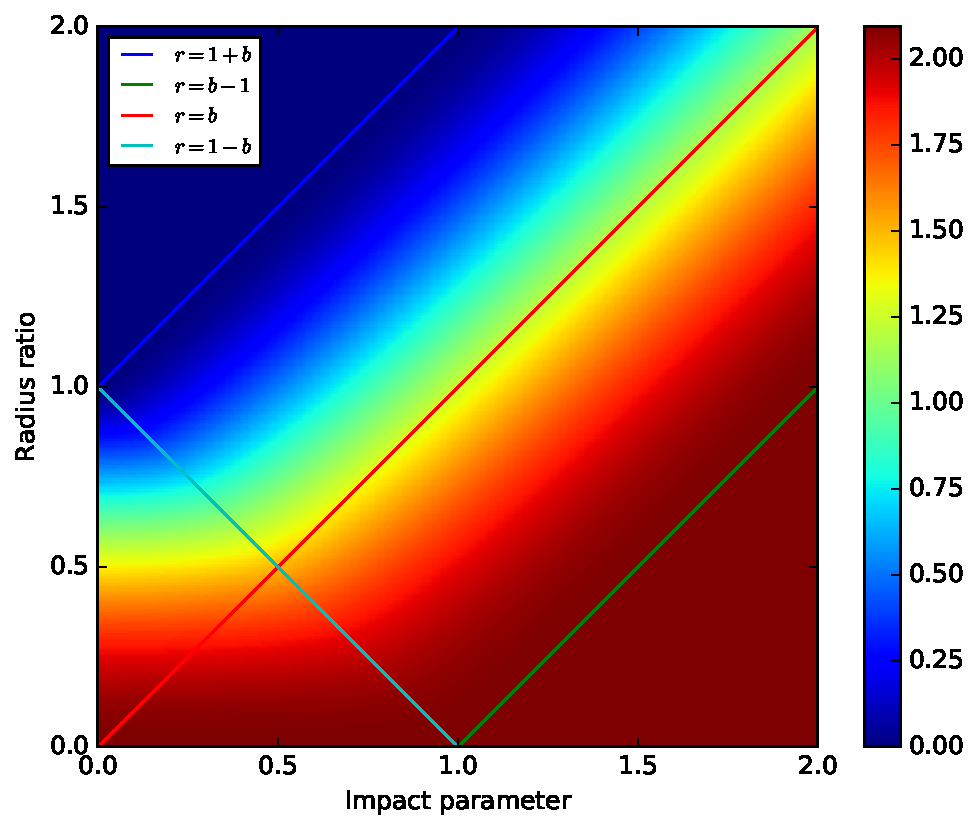
\includegraphics[width=0.8\linewidth]{figures/julia/transit_linear.pdf}
    \caption{The intensity of a linearly limb-darkened star ($u_1=1$) being
    eclipsed, $\mathfrak{s}_1(r,b)$.
    In the limit $b > r+1$, no eclipse occurs, so $\mathfrak{s}_1=1$.  For $b < r-1$, the star
    is completely eclipsed and $\mathfrak{s}_1=0$.  In the limits $b=r$ and $b=1-r$, special
    expressions must be used.
    \jlcodelink{transit_linear}\label{transit_linear}}
    \end{centering}
\end{figure}

\begin{figure}[p!]
    \begin{centering}
    \includegraphics[width=0.8\linewidth]{figures/julia/s2_residuals_MA2002.pdf}
    \caption{The numerical error in computing the flux of an eclipsed, linearly
             limb-darkened star ($u_1=1$) using the equations in \citet{MandelAgol2002}.
             \jlcodelink{s2_residuals_MA2002}\label{s2_plot_MA2002}}
    \end{centering}
\end{figure}

\begin{figure}[p!]
    \begin{centering}
    \includegraphics[width=0.8\linewidth]{figures/julia/s2_residuals.pdf}
    \caption{The numerical error in computing the flux of an eclipsed, linearly
    limb-darkened star ($u_1=1$) using the $\mathfrak{s}_1(r,b)$ formalism introduced in this
    paper. Compare to Figure~\ref{s2_plot_MA2002}, noting the change in the color
    scale. The new method is eight orders of magnitude more precise on average,
    approaching machine epsilon everywhere in the domain. 
    \jlcodelink{s2_residuals}\label{s2_plot}}
    \end{centering}
\end{figure}

\begin{figure}[p!]
    \begin{centering}
    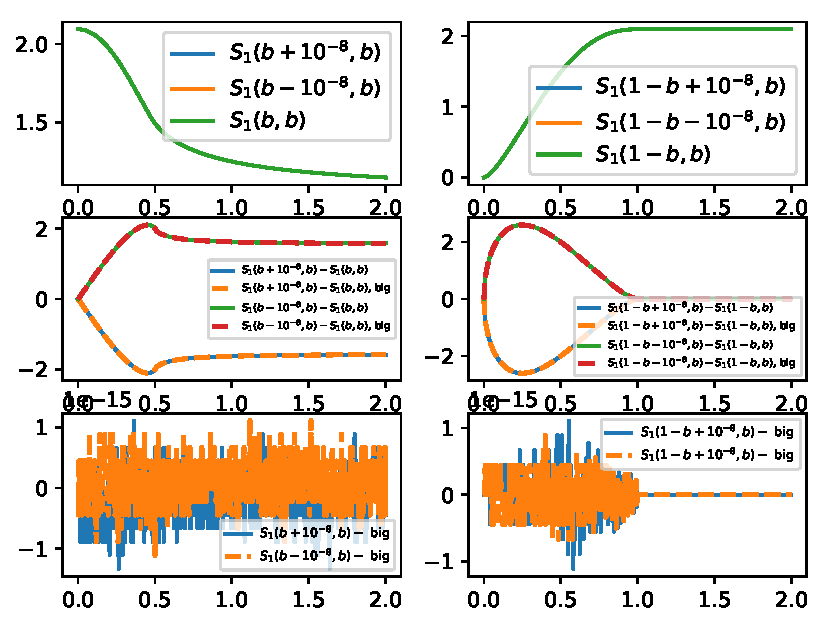
\includegraphics[width=\linewidth]{figures/julia/s2_machine.pdf}
    \caption{The accuracy of $\mathfrak{s}_1(r,b)$ near $b=r$ (left panel) and
    $b=1-r$ (right panel) for $\epsilon = 10^{-8}$. The $x$-axes are impact parameter $b$,
    while the $y$ axes in the top panels show $\mathfrak{s}_1(r,b)$, with $r$
    given in the legend of each panel. The middle panels plot
    the difference $(\mathfrak{s}_1(b,b\pm\epsilon)-\mathfrak{s}_1(b,b))/\epsilon$
    and $(\mathfrak{s}_1(b,1-b\pm\epsilon)-\mathfrak{s}_1(b,1-b))/\epsilon$. The bottom
    panels show the numerical precision by the comparing double precision
    computation with \texttt{BigFloat} precision (256-bit). \jlcodelink{s2_machine}\label{s2_machine}}
    \end{centering}
\end{figure}

\todo{This appears to be a dangling paragraph... Should this expression be in
terms of $\mathfrak{s}_0$ and $\mathfrak{s}_1$?}
From \citet{MandelAgol2002}, the total flux visible during the occultation of a
body whose surface map is given by $I(\upmu)/I(1) = 1 - u_1(1 - \upmu)$ may be computed
as
\begin{eqnarray}
\frac{F(u_1,r,b)}{F_0} &=& \frac{\pi(1-u_1)(1-\Lambda^e)+ u_1 \mathfrak{s}_1(r,b)}{\frac{2\pi}{3}u_1 + \pi(1-u_1)},\\
&=& 1-(1-u_1/3)^{-1}\left[(1-u_1)\Lambda^e(r,b) + u_1\left(\Lambda(r,b)+\tfrac{2}{3}\Theta(r-b)\right)\right],
\end{eqnarray}
where
and $F_0$ is the total unocculted flux.  % Note:  I'm not using this in
% transit_poly since it is not as precise as the starry expressions.

\subsection{Derivatives}

The expressions for the derivatives of the linear limb-darkening
light curve with respect to $r$ and $b$ are particularly simple:
%
\begin{proof}{biglam_deriv}
    \label{eq:dbiglam_dr}
    \frac{\partial \Lambda}{\partial r} &=
    \begin{dcases}
          0 & \qquad  r = 0\\
          0 & \qquad  \vert r- b\vert \ge 1\\
          2 r\sqrt{1-r^2} & \qquad b = 0\\
           \frac{2}{\pi} & \qquad b = r = \tfrac{1}{2}\\
          \frac{4r}{\pi} E(4r^2) & \qquad b= r < \tfrac{1}{2}\\
          \frac{2}{\pi} \mathrm{cel}(k_c,1,1,0) & \qquad b= r > \tfrac{1}{2}\\
          \frac{8r}{\pi}\sqrt{r(1-r)} & \qquad b+r =1\\
          \frac{8br^2 E(k^2) + 2r(1-(b+r)^2)K(k^2)}{\pi\sqrt{br}}
                    &\\ \phantom{XX}
          = \frac{1}{\pi\sqrt{br}}\mathrm{cel}(k_c,1,2r(1-(b-r)^2),0) & \qquad k^2 < 1
          %
          \\[1.5em]
          %
          \frac{4r}{\pi}\sqrt{1-(b-r)^2} E(k^{-2})
                    &\\ \phantom{XX}
          = \frac{4r}{\pi}\sqrt{1-(b-r)^2} \mathrm{cel}(k_c,1,1,k_c^2)& \qquad k^2 > 1\\
    \end{dcases}
\end{proof}
and
\begin{proof}{biglam_deriv}
    \label{eq:dbiglam_db}
    \frac{\partial \Lambda}{\partial b} &=
    \begin{dcases}
          0 & \qquad  r = 0\\
          0 & \qquad  \vert r- b\vert \ge 1\\
          0 & \qquad b = 0\\
           -\frac{2}{3\pi} & \qquad b = r = \tfrac{1}{2}\\
          \frac{4r}{3\pi}\mathrm{cel}(k_c,1,-1,k_c^2) & \qquad b= r < \tfrac{1}{2}\\
          -\frac{2}{3\pi} \mathrm{cel}(k_c,1,1,2k_c^2) & \qquad b= r > \tfrac{1}{2}\\
          -\frac{8r}{3\pi}\sqrt{r(1-r)} & \qquad b+r =1\\
           \frac{4r(r^2+b^2-1) E(k^2) + 2r(1-(b+r)^2)K(k^2)}{3\pi\sqrt{br}}
                    &\\ \phantom{XX}
          = \frac{1-(b-r)^2}{3\pi \sqrt{br}} \mathrm{cel}(k_c,1,-2r,(1-(b+r)^2)/b) & \qquad k^2 < 1
          %
          \\[1.5em]
          %
          \frac{2}{3b\pi}\sqrt{1-(b-r)^2}\left[(r^2+b^2-1) E(k^{-2}) +(1-(b+r)^2)K(k^{-2})\right]
                    &\\ \phantom{XX}
          =\frac{4r}{3\pi}\sqrt{1-(b-r)^2}\mathrm{cel}(k_c,1,-1,k_c^2) & \qquad k^2 > 1,\\
    \end{dcases}
\end{proof}
where we have given some of the expressions in terms of both the standard elliptic integrals
and the general elliptic integral.

% Note that if we had included the radius of the source star in these formulae,
% then the derivatives with respect to the radius of the star yield the
% transit light curve of a uniform, thin emission shell \citep{Schlawin2010}.

\todo{We need an equation here explicitly stating the derivatives of the $\mathfrak{s}_2$ term.}

We have tested these formulae with finite-difference derivatives evaluated at
256-bit precision, and, as with the total flux term, we find that these are accurate
to $\la 2 \times 10^{-15}$, close to machine precision.

We next increase the power of limb-darkening by one, $\upmu^2$.

\section{Quadratic limb-darkening}\label{sec:quadratic}

The next order of limb-darkening has been widely studied due to its
accurate description of stellar atmospheres \citep{Claret2000,MandelAgol2002,Pal2008}.
We summarize here the formulae for quadratic limb-darkening with $I(1)=1$, $u_1=2$ and
$u_2=-1$, so that $I(\mu)=\mu^2$, along with the derivatives, using the transformed 
expressions described above.  The general quadratic case may be computed as
a linear combination with the foregoing uniform and linear cases.

\todo{Split this into a separate section on derivatives, similar to the previous two cases.}

We first give the formula for the function $\eta(r,b)$, which is used in \citet{MandelAgol2002}, in
terms of quantities we have defined above for the uniform case:
\begin{proof}{Eta}
    \label{eq:eta}
    \eta(r,b) &=
    \begin{dcases}
          \frac{1}{2\pi}\left[\kappa_1+r^2(r^2+2b^2)\kappa_0-\frac{1}{2}(1+5r^2+b^2)A_{kite}\right]
          %
          & \qquad k^2 \le 1
          %
          \\[1.5em]
          %
          \frac{r^2}{2}(r^2+2b^2)
          %
          & \qquad k^2 > 1\\
    \end{dcases}
\end{proof}
As $\kappa_0$, $\kappa_1$, and $A_{kite}$ were already computed in the
uniform case, these quantities are reused in the quadratic computation.
The derivatives are given by:
\begin{proof}{Eta}
    \label{eq:detadr}
    \frac{\partial \eta}{\partial r} &=
    \begin{dcases}
          \frac{2r}{\pi}\left[(r^2+b^2)\kappa_0-2A_{kite}\right]
          %
          & \qquad k^2 \le 1
          %
          \\[1.5em]
          %
          2r(r^2+b^2)
          %
          & \qquad k^2 > 1\\
    \end{dcases}
\end{proof}
and
\begin{proof}{Eta}
    \label{eq:detadb}
    \frac{\partial \eta}{\partial b} &=
    \begin{dcases}
          \frac{1}{2b\pi}\left[4r^2b^2\kappa_0-2(1+b^2+r^2)A_{kite}\right]
          %
          & \qquad k^2 \le 1
          %
          \\[1.5em]
          %
          2br^2
          %
          & \qquad k^2 > 1\\
    \end{dcases}
\end{proof}

With this definition, then the quadratic term, $\mathfrak{s}_2(r,b)$ is given by
\begin{eqnarray}
\mathfrak{s}_2 &=& 2 \mathfrak{s}_0 + 4\pi \eta - 2\pi,\\
\frac{\partial \mathfrak{s}_2}{\partial r} &=& 2 \frac{\partial \mathfrak{s}_0}{\partial r} + 4\pi \frac{\partial \eta}{\partial r},\\
\frac{\partial \mathfrak{s}_2}{\partial b} &=& 2 \frac{\partial \mathfrak{s}_0}{\partial b} + 4\pi \frac{\partial \eta}{\partial b},
\end{eqnarray}
where $\mathfrak{s}_0$ and its derivatives are defined in Equations (\ref{eq:uniform})--(\ref{eq:dS0_drb}).
With the formulae for $\mathfrak{s}_0$, $\mathfrak{s}_1$, and $\mathfrak{s}_2$, the light curve and derivatives
of quadratic limb-darkening may be computed with Equations (\ref{eq:flux}) and 
(\ref{eq:derivatives}) given below.

Finally, we turn our attention to the general polynomial limb-darkening case,
$\upmu^n$ with $n > 2$.  As discussed in \citet{starry},
these terms may be expressed exactly as the sum of
spherical harmonics with $m=0$. However, it is possible to explot
the azimuthal symmetry of the limb darkening problem to 
derive far more efficient and accurate formulae, which we describe in the following section.

\section{Higher Order Limb Darkening}
\label{sec:higher_order}
% ------------------------------------------------------------------------------
% ------------------------------------------------------------------------------
% ==============================================================================

In analogy with the linear and quadratic
limb darkening laws, let us define the polynomial limb darkening law of
order $N$ as
%
%
\begin{align}
    \label{eq:polynomialld}
    \frac{I(\upmu)}{I_0} &= 1 - u_1 (1 - \upmu) - u_2 (1 - \upmu)^2 - 
                                ... - u_{N}(1 - \upmu)^{N} \nonumber \\
                          &= \sum_{i=0}^N u_i \sum_{j=0}^i 
                                \binom{i}{j} (-1)^{j + 1} \upmu^j
\end{align}
%
where $I_0 \equiv I(1)$, $u_0 \equiv -1$, and $\upmu$
is the cosine of the angle between the line of sight and the vector normal to 
the body's surface. In a right-handed Cartesian coordinate system centered 
on the body, with the $z$-axis pointing to the observer, 
\begin{equation}\label{eq:xyz}
\upmu(x, y) = z(x, y) = \sqrt{1 - x^2 - y^2}.
\end{equation}
%
%Although the foregoing analysis takes advantage of the existing formalism
%in \starry developed for occultation of spheres with arbitrary spherical harmonic
%brightness, the problem can be simplified significantly for the limb-darkening
%case due to the azimuthal symmetry assumed for a star.  This simplification
%leads to analytic expressions for the derivatives, which we find can be
%evaluated with greater speed and accuracy compared with automatic differentiation.
%
If we let $\bvec{u}$ be the column vector of limb darkening coefficients
$\bvec{u} \equiv (u_0 \ u_1 \ u_2 \ ... \ u_N)^\mathsf{T}$ 
and $\mubasis$ be the polynomial basis
$\mubasis \equiv (1 \ z \ z^2 \ ... \ z^N)^\mathsf{T}$, we may 
express Equation~(\ref{eq:polynomialld}) more compactly as the
dot product
%
\begin{align}
    \label{eq:polynomialld_vec}
    \frac{I(z)}{I_0} &= \mubasis^\mathsf{T} \bvec{u} .
\end{align}

Our task is to compute the flux, $F$, observed during an occultation by
integrating this function over the visible area of the disk:
%
\begin{align}
    \label{eq:occint}
    F &=
    \oiint I(z) \, \dd S
    \nonumber \\
    &= 
    I_0 \oiint \mubasis^\mathsf{T}(z) \, \dd S \, \bvec{u} \quad.
\end{align}
%
In general, the surface integral in Equation~(\ref{eq:occint}) is difficult---if not
impossible---to solve directly. As in \citet{starry}, we note that the problem
is made significantly more tractable if we first perform a change of basis
operation:
%
\begin{align}
    \label{eq:greensbasis}
    \gbasis \equiv \bvec{A} \mubasis
\end{align}
%
where, as in \citet{starry}, we refer to $\gbasis$ as the \emph{Green's basis},
which we define below. The matrix $\bvec{A}$ is a yet-to-be-defined 
linear transformation of the coefficients $\bvec{u}$.
%
%\todo{The notation in this section needs work. I need to go through this
%and carefully explain all symbols, define the Greens basis, the Greens
%functions, and make it clear to the reader what all this math is! We
%should make sure this section stands by itself, not relying too much on the
%definitions/explanations in starry.}
%
The total flux may now be written as
%
\begin{align}
    \label{eq:occint_greens}
    F &= I_0 \oiint \gbasis^\mathsf{T} (z) \, \dd S \, \bvec{A} \bvec{u} \nonumber \\
                &= I_0 \, \mathfrak{s}^\mathsf{T} \bvec{A} \bvec{u} \quad ,
\end{align}
%
where 
%
\begin{align}
    \label{eq:solution_vector}
    \mathfrak{s}^\mathsf{T} \equiv \oiint \gbasis^\mathsf{T} (z) \, \dd S
\end{align}
%
is the \emph{solution vector} first introduced in \S \ref{sec:uniform}.
Our task is now to find solutions to the integral (\ref{eq:solution_vector})
where $\gbasis$ is some complete basis of polynomials in $z$.

As in \citet{starry}, we use Green's theorem to re-express the surface
integral as a line integral over the boundary of the visible portion of
the occulted body's disk, $\bvec{r} = x \xhat + y \yhat$:
%
%
\begin{align}
    \label{eq:greens}
    \mathfrak{s} &=
    \oint \bvec{G} (z) \cdot \dd \bvec{r}
    \quad,
\end{align}
%  
where $\bvec{G}$ is a matrix whose $n^{\mathrm{th}}$ row is the
vector 
%
\begin{align}
    \label{eq:greens_n}
    \bvec{G}_n (z) = G_{n,x} (z) \, \xhat + G_{n,y} (z) \, \yhat \quad.
\end{align}
%
The components $G_{n,x}$ and $G_{n,y}$ are chosen such that
%
\begin{align}
    \label{eq:DGg}
    \bvec{D} \wedge \bvec{G}_n &\equiv \frac{\dd G_{n,y}}{\dd \x}
                                     - \frac{\dd G_{n,x}}{\dd \y} \nonumber \\
                               &= \gbasisn(z) \quad.
\end{align}
%
As in \citet{Pal2012} and \citet{starry}, the operation 
$\bvec{D} \wedge \bvec{G}_n$ denotes the
\emph{exterior derivative} of $\bvec{G}_n$.
%
%
%Since the polynomial expansion only depends on $\upmu = z =\sqrt{1-x^2-y^2}$,
%where $(x,y,z)$ are the coordinates of the unit sphere, we only require
%Green's functions whose curl has dependence on $z$ for axially-symmetric
%limb-darkening.  
%
Following \citet{starry}, we choose the following form for 
Equation~(\ref{eq:greens_n}):
%
\begin{equation}
\mathbf{G}_n(z) = z^n (-y \xhat + x \yhat) \quad,
\end{equation}
%
yielding the following expression for the components of the Green's basis:
%
\begin{align}
\gbasisn(z)   &= \frac{\dd {G_n}_y}{\dd \x} - \frac{\dd {G_n}_x}{\dd \y} \nonumber \\[0.5em]
              &= 2 z^n + \frac{dz^n}{dz} \frac{z^2-1}{z} \nonumber \\[0.5em]
              &= \frac{1}{z} \frac{d}{dz}\left[ z^n(z^2-1)\right] \nonumber \\[0.5em]
              &= (n+2)z^n-n z^{n-2}
\end{align}
%
for $2 \le n \le N$. For the first two terms, we choose $\tilde{\mathfrak{g}}_0 = 1$
(uniform limb darkening) and $\tilde{\mathfrak{g}}_1 = z$ (linear limb darkening),
which we previously discussed in \S\ref{sec:uniform} and \S\ref{sec:reparam}.

% MENTION THIS LATER: Note that the total flux of each term in this basis set, $\tilde{\mathfrak{g}}_n$, integrates
% to zero for $2 \le n \le N$.

\todo{The contents of section 5.1 should go here.}

Returning to \eq{greens}, we may write the $n^\mathrm{th}$ component of 
the solution vector as
%
\begin{align}
    \label{eq:sn}
    \mathfrak{s}_n &= \mathcal{Q}(\bvec{G}_n) - \mathcal{P}(\bvec{G}_n)
    \quad,
\end{align}
%
where, as in \citet{Pal2012} and \citet{starry}, we define the \emph{primitive integrals}
%
\begin{align}
    \label{eq:primitiveP}
    \mathcal{P}(\bvec{G}_n) &=
    \int\displaylimits_{\pi-\phi}^{2\pi + \phi}
        \big[ G_{n,y}(r c_\varphi, b + r s_\varphi) c_\varphi -
              G_{n,x}(r c_\varphi, b + r s_\varphi) s_\varphi \big] r \dd \varphi
    \\
    %
\intertext{and}
    %
    \label{eq:primitiveQ}
    \mathcal{Q}(\bvec{G}_n) &=
    \int\displaylimits_{\pi-\lambda}^{2\pi + \lambda}
        \big[ G_{n,y}(c_\varphi, s_\varphi) c_\varphi -
              G_{n,x}(c_\varphi, s_\varphi) s_\varphi \big] \dd \varphi
    \quad,
\end{align}
%
%
where we defined
$c_\varphi \equiv \cos \varphi$
and
$s_\varphi \equiv \sin \varphi$
and we used the fact that along the arc of a circle,
%
\begin{align}
    \label{eq:dr}
    \dd \bvec{r} &= -r s_\varphi \, \dd \varphi \, \xhat +
                     r c_\varphi \, \dd \varphi \, \yhat
    \quad.
\end{align}
%
In Equations~(\ref{eq:primitiveP}) and (\ref{eq:primitiveQ}), $\mathcal{P}(\bvec{G}_n)$
is the line integral along the arc of the occultor of radius $r$,
and $\mathcal{Q}(\bvec{G}_n)$ is the line integral along the arc of the occulted
body of radius one.

\todo{Define $\lambda$ and $\phi$.  These are given by $\phi = \kappa_0-\pi/2$ and
$\lambda = \pi/2 - \kappa_1$.}

\todo{Work on the transition here. This section still doesn't flow well.}


This choice of Green's function yields particularly simple form for the primitive integrals of
\begin{align}
    \label{eq:primitiveP}
    \mathcal{P}(\bvec{G}_n) &=
    \int\displaylimits_{\pi-\phi}^{2\pi + \phi} z^n (r+b \sin{\varphi}) r d\varphi
    %
\intertext{and}
    %
    \label{eq:primitiveQ}
    \mathcal{Q}(\bvec{G}_n) &=
    \int\displaylimits_{\pi-\lambda}^{2\pi + \lambda} z^n d \varphi
\end{align}

Also, with this choice of basis, the primitive integral $\mathcal{Q}(\bvec{G}_n) = 0$ for
$1 \le n \le N$ since $z=0$ at the boundary of the star.   The $n=0$ case we have already
solved for uniform limb-darkening, and so it remains to find $\mathcal{P}(\bvec{G}_n)$.

The primitive integral
$\mathcal{P}(\bvec{G}_n)$ can be rewritten as
\begin{equation}
\mathcal{P}(\bvec{G}_n) =
\int_{\pi-\phi}^{2\pi + \phi} \left(1-r^2-b^2-2br s_\varphi\right)^{\frac{n}{2}} (r+b s_\varphi) r d\varphi,
\end{equation}
where $s_\varphi = \sin{\varphi}$.
We make the transformation $\xi = \tfrac{1}{2} \left(\varphi - \tfrac{3\pi}{2}\right)$, yielding
\begin{equation}\label{eq:greens_transformed}
\mathcal{P}(\bvec{G}_n) =
2r (4br)^{\frac{n}{2}}\int\displaylimits_{-\tfrac{\kappa_0}{2}}^{\tfrac{\kappa_0}{2}}
(k^2-\sin^2\xi)^{\tfrac{n}{2}} (r-b + 2b \sin^2 \xi) d\xi,
\end{equation}
for $2 \le n \le N$, where $\kappa_0 = 2 \sin^{-1}k$ for $k^2 \le 1$ and
$\kappa_0 = \pi$ for $k^2 > 1$.  We
reuse the value of $\kappa_0$ which was computed in the uniform limb-darkening
case (\S \ref{sec:uniform}).

With these integrals defined, the basis functions for the lightcurve are given
by $\mathfrak{s}_n$, where $\mathfrak{s}_0$ is given for uniform limb-darkening
in section \ref{sec:uniform}, $\mathfrak{s}_1$ is given by the linear limb-darkened
solution from section \ref{sec:reparam}, and  $\mathfrak{s}_n = \mathcal{Q}(\bvec{G}_n)
- \mathcal{P}(\bvec{G}_n) = -\mathcal{P}(\bvec{G}_n)$ for $2 \le n \le N$;
we have already given an alternate expression for $\mathfrak{s}_2$ in section \ref{sec:quadratic}.

We can express $\mathcal{P}(\bvec{G}_n)$ in terms of a sequence of integrals,
$\mathcal{M}_n(r,b)$, given by:
\begin{equation}\label{eq:M_of_n}
\mathcal{M}_n(r,b) = (4br)^{n/2} \int_{-\kappa_0/2}^{\kappa_0/2} (k^2-\sin^2\xi)^{\tfrac{n}{2}} d\xi,
\end{equation}
in terms of which the primitive integral takes the particulary simple form
\begin{proof}{pofgn_v01}\label{eq:primitive}
\mathcal{P}(\bvec{G}_n) = (1+r^2-b^2)\mathcal{M}_n - \mathcal{M}_{n+2}.
\end{proof}

The integrals $\mathcal{M}_n$ obey straightforward recursion relations
\begin{proof}{Mn_recursion}\label{eq:Mn_recursion}
%\begin{eqnarray}
\mathcal{M}_n &= \frac{1}{n} \left[ 2(n-1) (1-r^2-b^2) \mathcal{M}_{n-2} \right.\nonumber\\ 
  &+ \left. (n-2) (1-(b-r)^2)((b+r)^2-1) M_{n-4}\right],\\[1em]
\mathcal{M}_n &= \frac{(n+4)\mathcal{M}_{m+4} - 2(n+3)(1-r^2-b^2)\mathcal{M}_{n+2}}{(n+2)(1-(b-r)^2)((b+r)^2-1)},
%\end{eqnarray}
\end{proof}
where the first relation may be used for upwards recursion in $n$ for $k^2 > \frac{1}{2}$, 
and the second for downward recursion in $n$ otherwise.
In practice we replace $\mathcal{M}_{n+2}$ in Equation~(\ref{eq:primitive}) with 
the recursion relation to obtain a more stable expression for $\mathcal{P}(\bvec{G}_n)$:
\begin{proof}{pofgn_v02}\label{eq:PofGn_v02}
\mathcal{P}(\bvec{G}_n) = 2r^2 \mathcal{M}_n - \frac{n}{n+2}\left((1-r^2-b^2)\mathcal{M}_n+(1-(b-r)^2)((b+r)^2-1)\mathcal{M}_{n-2}\right).
\end{proof}

Note that these recursion relations involve every fourth term, so we need to compute
the first four terms analytically.  These are given by:
\begin{proof}{Mn_initial}
\mathcal{M}_0 &= \kappa_0,\nonumber\\
\mathcal{M}_1 &= 2 (4br)^{1/2} \left[E(k^2)-(1-k^2)K(k^2)\right],\nonumber\\
\mathcal{M}_2 &= 4br\left[(k^2-\tfrac{1}{2}) \kappa_0 + k\sqrt{1-k^2}\right],\nonumber\\
\mathcal{M}_3 &= \tfrac{2}{3}(4br)^{3/2} \left[(4k^2-2)E(k^2)+(3k^2-2)(k^2-1)K(k^2)\right],
\end{proof}
for $k^2 \le 1$, while for $k^2 > 1$,
\begin{proof}{Mn_initial}
\mathcal{M}_0 &= \pi,\nonumber\\
\mathcal{M}_1 &= 2(1-(r-b)^2)^{1/2}E(k^{-2}),\nonumber\\
\mathcal{M}_2 &= \pi(1-b^2-r^2),\nonumber\\
\mathcal{M}_3 &= \tfrac{2}{3}(4br)^{3/2} k^3\left[2(2-k^{-2})E(k^{-2})-(1-k^{-2})K(k^{-2})\right].
\end{proof}
%
%
We re-express the elliptic integrals for $n=1$ and $n=3$ in terms of the cel integrals which
were already computed for the linear limb-darkening case,
\begin{proof}{Mn_cel}
\mathcal{M}_1 &= 2 (4br)^{1/2} k^2 \mathrm{cel}(k_c,1,1,0),\nonumber\\
\mathcal{M}_3 &= \tfrac{2}{3}(4br)^{3/2}k^2 \left[ \mathrm{cel}(k_c,1,1,k_c^2)+(3k^2-2) \mathrm{cel}(k_c,1,1,0)\right],
\end{proof}
for $k^2 \le 1$, while for $k^2 > 1$,
\begin{proof}{Mn_cel}
\mathcal{M}_1 &= 2(1-(r-b)^2)^{1/2} \mathrm{cel}(k_c,1,1,k_c^2),\nonumber\\
\mathcal{M}_3 &= \tfrac{2}{3}(1-(b-r)^2)^{3/2} \left[(3-2k^{-2}) \mathrm{cel}(k_c,1,1,k_c^2)+k^{-2} \mathrm{cel}(k_c,1,1,0\right].
\end{proof}
where, as before, $k_c = \sqrt{1-k^2}$ for $k^2 \le 1$, and $k_c = \sqrt{1-k^{-2}}$ for $k^2 > 1$.

For downward recursion, we compute the top four $\mathcal{M}_n$ expressions, $N-3 \le n \le N$,
in terms of series expansions.
When $k^2 \le 1$, the integrals may be expressed in terms of the following
Hypergeometric functions and infinite series,
\begin{proof}{Mn_series}\label{eq:Mn_series}
\mathcal{M}_n &= (4br)^{n/2} k^{n+1} \pi^{1/2} \frac{\Gamma{(1+\tfrac{n}{2})}}{\Gamma(\tfrac{3}{2}+\tfrac{n}{2})} \,_2F_1(\tfrac{1}{2},\tfrac{1}{2};\tfrac{3}{2}+\tfrac{n}{2};k^2),\nonumber\\
&= (1-(r-b)^2)^{n/2} k \sum_{j=0}^{j_{max}} \alpha_j k^{2j},\nonumber\\
\alpha_0 &= \sqrt{\pi} \frac{\Gamma(1+\tfrac{n}{2})}{\Gamma(\tfrac{3}{2}+\tfrac{n}{2})},\nonumber\\
\alpha_j &= \alpha_{j-1} \frac{(2j-1)^2}{2j(1+n+2j)}.
\end{proof}
Although $j_{max} = \infty$, in practice we set $j_{max} = 100$, and the series is 
truncated when a term goes below a tolerance specified by the numerical precision.

We find that upward recursion in $n$ is more stable for $k^2 > \tfrac{1}{2} $,
while downward recursion is more stable for $k^2 < \tfrac{1}{2}$.  Note that
this differs from \starry for which downward recusion was also required for $k^2 > 2$.

With the computation of the light curves for the basis functions, $\mathfrak{s}_n$, the final step is to
combine these to make the full light curve with limb-darkening coefficients, which we describe
next.

\subsection{Limb-darkening coefficients}

Our expansion for limb-darkening in terms of $u_n(1-\upmu)^n$ (Equation \ref{eq:polynomialld}) needs to
be re-expressed in terms of the Green's basis terms $d_n \left[(n+2)\upmu^n -n \upmu^{n-2}\right]$,
where $d_n$ are constants.
We accomplish this by first transforming $u_n$ to coefficients of $a_n \upmu^n$,
and then transforming from $a_n$ to $d_n$.

\todo{Rodrigo, you wanted to change notation from $d_n$ to $g_n$?}

We rewrite $I(\upmu)$ in terms of these three expansions
\begin{eqnarray}
\frac{I(\upmu)}{I(1)} &=& 1 - \sum_{i=1}^N u_i \sum_{j=0}^i \binom{i}{j} (-1)^j \upmu^j,\nonumber\\
&=& \sum_{n=0}^N a_n \upmu^n,\nonumber\\
&=& d_0 + d_1 \upmu + \sum_{n=2}^N d_n \left[(n+2)\upmu^n -n \upmu^{n-2}\right].
\end{eqnarray}
Note that $a_0 \equiv 1-\sum_{n=1}^N a_n = 1 - \sum_{i=1}^N u_i$ in the formalism of \citet{Gimenez2006}.
The transformation between $u_n$ and $a_n$ is straightforward based on
looping over the binomial expansion of each of the $u_n$ terms (Equation \ref{eq:polynomialld}),
for example $a_1 = \sum_{n=1}^N n u_n$, while in general
\begin{equation}\label{eq:an_of_un}
a_n = -\sum_{i=n}^N u_i \binom{i}{n}(-1)^n,
\end{equation}
for $1 \le n \le N$.
Then, with the computed $a_n$ values, we can find $d_n$ from downward recursion
using the relation
\begin{equation} \label{eq:dn_of_an}
d_n = \frac{a_n}{n+2} + d_{n+2},
\end{equation}
starting with $n=N$, with $d_{N+1}=d_{N+2}=0$.

The total light curve is computed from
\begin{eqnarray}\label{eq:flux}
\mathcal{F} &=& \frac{F}{F_0} = \frac{1}{F_0}\sum_{n=0}^N d_n \mathfrak{s}_n,\\
F_0 &=& \pi(d_0+ \tfrac{2}{3} d_1),
\end{eqnarray}
where $F_0$ is the unobscured flux, and $\mathcal{F}$ is the flux normalized
such that the unobscured flux is unity.

Note that the unobscured flux for each basis function (for $b \ge 1+r$ or $r=0$) is zero for
all $\mathfrak{s}_n(r,b)$ with $2 \le n \le N$, which is why the total unobscured flux,
$F_0$, only depends upon $d_0$ and $d_1$.

\subsection{Analytic derivatives}\label{sec:analytic_derivatives}

The derivatives of $\mathcal{P}(\bvec{G}_n)$ may be expressed simply as functions
of $\mathcal{M}_n$:
\begin{eqnarray}
\frac{\partial \mathcal{P}}{\partial r} &=& 2r \left[(n+2)\mathcal{M}_n - n \mathcal{M}_{n-2}\right],\\
\frac{\partial \mathcal{P}}{\partial b} &=& \frac{n}{b} \left[(r^2+b^2)(\mathcal{M}_n - \mathcal{M}_{n-2})+(r^2-b^2)^2\mathcal{M}_{n-2}\right].
\end{eqnarray}

We find that the derivative with respect to impact parameter becomes numerically
unstable for small values of $b$ due to cancellation between the two
terms, followed by division by $b$.  To avoid this problem
for small $b$, we have derived an alternative expression which we utilize when
$b < b_c$, where $b_c$ is a (small) cutoff value, which avoids division by $b$:
\begin{eqnarray}
\frac{\partial \mathcal{P}}{\partial b} = n \left[b\mathcal{M}_n +(2r^3+b^3-3r^2b-b-3) \mathcal{M}_{n-2}-4r^3\mathcal{N}_{n-2}\right],
\end{eqnarray}
where we have defined a new integral, $\mathcal{N}_n$,
\begin{equation}\label{eq:N_of_n}
\mathcal{N}_n(r,b) = (4br)^{n/2} \int_{-\kappa_0/2}^{\kappa_0/2} (k^2-\sin^2\xi)^{\tfrac{n}{2}} \sin^2{\xi} d\xi,
\end{equation}
which obeys the recursion relation
\begin{proof}{Nn_recursion}
\mathcal{N}_n = \frac{1}{n+2} \left[\mathcal{M}_n + n(1-(b+r)^2) \mathcal{N}_{n-2}\right].
\end{proof}
Since this recursion relation involves every other term, we only need the two lowest terms,
which are given by:
\begin{proof}{Nn_cel}
\mathcal{N}_0 &= \tfrac{1}{2}\kappa_0 - k k_c,\nonumber\\
\mathcal{N}_1 &= \tfrac{2}{3}(4br)^{1/2} k^2 \left[-\mathrm{cel}(k_c,1,1,k_c^2) + 2 \mathrm{cel}(k_c,1,1,0)\right],
\end{proof}
for $k^2 \le 1$ and
\begin{proof}{Nn_cel}
\mathcal{N}_0 &= \frac{\pi}{2},\nonumber\\
\mathcal{N}_1 &=  \tfrac{2}{3}(4br)^{1/2} k \left[2\mathrm{cel}(k_c,1,1,k_c^2) - \mathrm{cel}(k_c,1,1,0)\right],
\end{proof}
for $k^2 > 1$.

In the $k^2 < \tfrac{1}{2}$ limit, we find the upward recursion to be unstable, and so we evaluate the expressions for $\mathcal{N}_{N}$ and $\mathcal{N}_{N-1}$
with a series solution (as we did for $\mathcal{M}_{N-3}$,...,$\mathcal{M}_N$),
\begin{proof}{Nn_series}\label{eq:Nn_series}
\mathcal{N}_n &= (4br)^{n/2} k^{n+3} \frac{\pi^{1/2}}{2} \frac{\Gamma{(1+\tfrac{n}{2})}}{\Gamma(\tfrac{5}{2}+\tfrac{n}{2})} \,_2F_1(\tfrac{1}{2},\tfrac{3}{2};\tfrac{5}{2}+\tfrac{n}{2};k^2),\nonumber\\
&= (1-(r-b)^2)^{n/2} k^3 \sum_{j=0}^{j_{max}} \gamma_j k^{2j},\nonumber\\
\gamma_0 &= \frac{\sqrt{\pi}}{2} \frac{\Gamma(1+\tfrac{n}{2})}{\Gamma(\tfrac{5}{2}+\tfrac{n}{2})},\nonumber\\
\gamma_j &= \gamma_{j-1} \frac{(4j^2-1)}{2j(3+n+2j)}.
\end{proof}
We then use downward recursion with the relation
\begin{equation}
\mathcal{N}_n = \frac{(n+4)\mathcal{N}_{n+2} - \mathcal{M}_{n+2}}{(n+2)(1-(b+r)^2)},
\end{equation}
to iterate down to $n=3$, while finally computing $n=1$ and $n=2$ exactly.

Evaluating this additional integral adds further computational expense, but in
practice we only need to compute it for $b < b_c = 10^{-3}$ to obtain similar accuracy
to the other expressions.  This is encountered rarely as it only applies when the
occultor is nearly aligned with the source.

With the computation of $\mathfrak{s}_n = -\mathcal{P}(\bvec{G}_n)$, we then
compute the derivatives of the light curve as
\begin{eqnarray}
\frac{\partial \mathfrak{s}_n}{\partial r} &= & -\frac{\partial \mathcal{P}(\bvec{G}_n)}{\partial r},\\
\frac{\partial \mathfrak{s}_n}{\partial b} &= & -\frac{\partial \mathcal{P}(\bvec{G}_n)}{\partial b},
\end{eqnarray}
for $2 \le n \le N$, while the $n=0$ and $n=1$ terms are handled separately as in
section \ref{sec:reparam}.

The derivatives of the normalized flux, $\mathcal{F}$, as a function of $r$, $b$, and
$d_n$ are then computed as
\begin{eqnarray}\label{eq:derivatives}
\frac{\partial \mathcal{F}}{\partial r} &=& \sum_{n=0}^N\frac{ d_n}{F_0} \frac{\partial \mathfrak{s}_n}{\partial r},\\
\frac{\partial \mathcal{F}}{\partial b} &=& \sum_{n=0}^N\frac{ d_n}{F_0} \frac{\partial \mathfrak{s}_n}{\partial b},\\
\frac{\partial \mathcal{F}}{\partial d_0} &=&  -\frac{\pi \mathcal{F}}{F_0} + \frac{\mathfrak{s}_0}{F_0},
\end{eqnarray}
\begin{eqnarray}
\frac{\partial \mathcal{F}}{\partial d_1} &=&  -\frac{2\pi \mathcal{F}}{3F_0} +\frac{\mathfrak{s}_1}{F_0},\\
\frac{\partial \mathcal{F}}{\partial d_n} &=&  \frac{\mathfrak{s}_n}{F_0},
\end{eqnarray}
where the last line is for $2 \le n \le N$.

The derivatives of the coefficients, $\frac{\partial d_j}{\partial u_i}$, are
computed by differentiating each term in Equation~(\ref{eq:an_of_un}) to obtain
$\frac{\partial a_n}{\partial u_i}$, and differentiating each term in Equation~(\ref{eq:dn_of_an})
 to obtain $\frac{\partial d_j}{\partial a_n}$, and propagating 
the derivatives via the chain rule.  Then, the light curve derivatives are given by
\begin{eqnarray}\label{eq:dFdu}
\frac{\partial \mathcal{F}}{\partial u_i} =  \sum_{j} \frac{\partial d_j}{\partial u_i}\frac{\partial \mathcal{F}}{\partial d_j}.
\end{eqnarray}

With the description of the light curve computation complete, we next discuss
the integration of the light curve over a finite time step.

\section{Time integration} \label{sec:time}

Given that most observations are made over a finite exposure time,
the integration of the light curve over time is necessary for representing
a transit light curve with high fidelity \citep{Kipping2010}.  For constructing
a light curve, usually one divides the fluence by the integration time
to obtain the time-averaged flux.  For optimizing and inferring the 
posterior of model parameters, we would like to compute the derivatives
of the time-averaged flux with respect to the model parameters.

The instantaneous flux is a function of $3+n$ parameters in the Green's basis, 
$\{r,b,d_n\}$, or $2+n$ parameters in the polynomial in $1-\upmu$ basis, and of
these, only one varies with time, $b(t)$.  Thus, we can compute the time-
dependent flux with a model for $b(t)=b(\bvec{x},t)$, where
where $b(\bvec{x},t)$ is a model for the impact parameter as a function of time
and model parameters $\bvec{x}$.  The set of model parameters need to be specified
by a function, which, for example, might be a Keplerian orbit of the two bodies
with respect to one another, or a full dynamical model of an n-body system.
To compute the derivatives of the light curve with respect to $\bvec{x}$, the
derivatives of the dynamical model must be computed as well.

The time-averaged flux, $\overline{\mathcal{F}}$, and its derivatives, are given by 
\begin{eqnarray}\label{eq:avg_flux}
\overline{\mathcal{F}} &=& \frac{1}{\Delta t} \int_{t-\tfrac{1}{2}\Delta t}^{t+\tfrac{1}{2}\Delta t} \mathcal{F}(t^\prime) dt^\prime,\\
\frac{\partial \overline{\mathcal{F}}}{\partial r} &=& \frac{1}{\Delta t} \int_{t-\tfrac{1}{2}\Delta t}^{t+\tfrac{1}{2}\Delta t} \frac{\partial \mathcal{F}(t^\prime)}{\partial r} dt^\prime,\\
%\frac{\partial \overline{\mathcal{F}}}{\partial b}&=& \frac{1}{\Delta t} \int_{t-\tfrac{1}{2}\Delta t}^{t+\tfrac{1}{2}\Delta t} \frac{\partial \mathcal{F}(t^\prime)}{\partial b} dt^\prime,\\
\frac{\partial \overline{\mathcal{F}}}{\partial d_i}&=& \frac{1}{\Delta t} \int_{t-\tfrac{1}{2}\Delta t}^{t+\tfrac{1}{2}\Delta t} \frac{\partial \mathcal{F}(t^\prime)}{\partial d_i} dt^\prime,\\
\frac{\partial \overline{\mathcal{F}}}{\partial \bvec{x}} &=& \frac{1}{\Delta t}
\int_{t-\tfrac{1}{2}\Delta t}^{t+\tfrac{1}{2}\Delta t} \frac{\partial \mathcal{F}}{\partial b}\frac{\partial b(t^\prime)}{\partial \bvec{x}} dt^\prime,
\end{eqnarray}
where $t$ is taken to be the mid-point of the transit exposure time, and
$\Delta t$ is the exposure time.

As an example, we choose the approximate transit model $b(t) = (b_0^2 + v^2(t-t_0)^2)^{1/2}$,
which ignores acceleration and curvature during a transit, and thus is valid in the
limit of large orbital separation.  We compute the time-averaged flux and derivatives 
with respect to $\bvec{x} = \{t_0,v,b_0\}$ for a length of integration time $\Delta t$.
\todo{Update this description of the time-integration.}
The integration is carried out with an adaptive refinement of the exposure time interval by
factors of two until the midpoint in each refined interval is within $10^{-6}r^2$
of the mean of the start and end with a maximum
number of refinement depths of 32.  Figure \ref{fig:integrated_derivs} shows a
comparison of the derivatives of the time-integrated light curve for this
impact parameter model.  

The time-integration smooths both the features of
the light curve, as well as the features of the derivative curves.  The similarity of
the shape of the derivative with respect to $v$ and $b_0$ makes it apparent
that there may be partial degeneracies between the impact parameter and duration
of a transit, which can make the impact parameter more difficult to measure, especially 
when the exposure time is longer than the time of ingress/egress.  Likewise, the
derivatives with respect to the two limb-darkening parameters have a similar shape,
which explains why in some cases it can be difficult to constrain both parameters.

\begin{figure}
    \begin{centering}
    \includegraphics[width=\linewidth]{figures/julia/integrate_transit_gradient.pdf}
    \caption{Comparison of the normalized flux and its derivatives with (solid) and
    without (dashed) time-integration.  The integration time is indicated in the
    upper left panel with a horizontal blue line. The derivatives are computed with
    respect to $\{r,t_0,v,b_0,u_1,u_2\}$.  The parameters are given by $r=0.1$,
    $t_0 = 0$, $b_0=0.5$, $u_1=u_2=0.3$. \jlcodelink{integrate_transit_gradient}
    \label{fig:integrated_derivs}}
    \end{centering}
\end{figure}

This completes the description of the light curve computation, along
with its derivatives.  We now turn to discussing the implementation of
the computation, followed by comparison with existing codes.

\section{Implementation details}

There are several details in our implementation of the foregoing equations
which give further speedup of the computation, which we describe in this
section.

When a light curve is computed, there are some computations which only
need to be carried out once, and then reused at each time step in the
light curve computation.  
We define a structure to hold the variables
which are reused throughout the light curve.  In addition, due to the greater 
computational expense of square-roots and divisions, where possible we try 
to only compute a square root or division once, storing these in a variable
within the structure, and then reusing these with cheaper multiplication 
throughout the computation when needed.  For instance, for many formulae we 
require the inverse of an integer, so an array of integer inverses is computed 
once and stored, and then accessed as required rather than recomputed.

Once the number of limb-darkening
terms, $N$, is specified, then the series coefficients for $\mathcal{M}_n$
and $\mathcal{N}_n$, $\alpha_j$ and $\gamma_j$, are a simple function of $j$ 
and $n$, and so we compute these coefficients once, and store them in a vector 
for $k^2 \le 1$, separately for $N-3$ to $N$ for $\mathcal{M}_n$, and for 
$N-1$ and $N$ for $\mathcal{N}_n$.

In addition, once $N$ is specified, then the transformation matrix for
the Jacobian from $d_i$ to $u_j$, $\frac{\partial d_i}{\partial u_j}$,  
remains the same throughout the light curve 
computation, so we compute this matrix only once, and then compute the
flux derivative (Equation \ref{eq:dFdu}) with matrix multiplication.
In fact, since the Jacobian matrix for transforming the derivatives from $d_i$
to $u_j$ can be expensive to apply, we can carry out the gradient of the 
likelihood function with respect to $d_i$, and then apply the Jacobian 
transformation from $d_i$ to $u_j$ only once to obtain the gradient
of the likelihood with respect to the limb-darkening parameterization.
In practice, we are usually only concerned with optimizing a likelihood
or computing gradients of a likelihood for Hamiltonian Markov Chain
Monte Carlo, so the derivatives of the particular points in the
light curve with respect to $u_i$ aren't needed.  This results in a
significant computational savings, especially for large $N$.
Transformation to other parameterizations, such as $q_1$ and $q_2$
defined by \citet{Kipping2013}, may also be accomplished after the
fact by applying the Jacobian to compute the gradient of the likelihood 
in terms of these transformed parameters.

In computing the elliptic integrals, cel, we found that several terms
which appear in the Bartky formalism are repeated amongst all three elliptic 
integrals which appear in the expressions for $\mathfrak{s}_1$.  Consequently, we carry 
out a parallel computation of these elliptic integrals such that these
repeated terms are only computed once;  this improves the efficiency of
the elliptic integral computation.  Once these elliptic integrals
are computed for $\mathfrak{s}_1$, the elliptic integrals $\mathrm{cel}(k_c,1,1,k_c^2)=E(m_k)$
and $\mathrm{cel}(k_c,1,1,0)=(E(m_k)-(1-m_k)K(m_k))/m_k $ are
stored in the structure and reused for computing $\mathcal{M}_n$
and $\mathcal{N}_n$.

We find that the precision of the computation begins to degrade for
$N \approx 25-30$.  For large values of $N$, the computing time for
propagating the derivatives from $d_i$ to $u_i$ scales as $N^2$, and
thus can dominate the computation time.  We utilize the BLAS linear
algebra library (specifically, the routine \texttt{gemv}) for efficient 
multiplication of this matrix times the derivative of the light curve with 
respect to $d_i$ in order to obtain the derivatives with respect to $u_i$.
However, as we note above, an even more efficient approach is to
simply apply this transformation once to the gradient of the likelihood.

\section{Benchmarking}\label{sec:benchmark}

We have measured the performance of the limb-darkened light curves
with derivatives as a function of the number of computed data points
and as a function of the number of limb-darkening coefficients.  We
have computed the timing for $r=0.1$ and for a number of impact
parameters ranging from $10^2$ to $10^6$, and the number of limb-darkening
coefficients ranging from $1$ to $144$.  For each set of timing benchmark
parameters, we carried out nine measurements  of the timing, and
we use the median of these for plotting purposes.  The benchmarking
for the \texttt{Julia} code was carried out with \texttt{v0.7} of
Julia on a MacBook Pro with 2.8 GHz Intel Core i7.
No sub-sampling was carried out in this computation.

Figure \ref{fig:ncoeff} shows that the time dependence is linear with the
number of $b$ values (which is equivalent to the number of data points
in the light curve).  The linear scaling with time holds for each value of
the number of limb-darkening coefficients.

Figure \ref{fig:nlimb} shows that the time dependence scales approximately
as $N^{0.2-1}$.  As with the number of light-curve points, we have taken
the median over nine measurements for each set of parameters.  We then
scaled the timing to the single-coefficient case, and took a second
median over the number of light curve points as the cube-root scaling scales
about the same with different numbers of points in the light curve.

\begin{figure}
    \begin{centering}
    \includegraphics[width=\linewidth]{figures/julia/benchmark_transit_poly.pdf}
    \caption{Scaling of the computation time in seconds with the number of
    data points in the light curve for $r=0.1$ with $b$ ranging from $0$ to $1.2$,
    and with the number of limb-darkening coefficients, $N$. \jlcodelink{benchmark_transit_poly}
    \label{fig:ncoeff}}
    \end{centering}
\end{figure}

\begin{figure}
    \begin{centering}
    \includegraphics[width=\linewidth]{figures/julia/benchmark_limbdark_timing.pdf}
    \caption{Scaling of the computation time with the number of
    limb-darkening coeffients, $N$.  The $y$-axis scales the timing with respect
    to the timing for a single limb-darkening coefficient. \jlcodelink{benchmark_transit_poly}
    \label{fig:nlimb}}
    \end{centering}
\end{figure}

\section{Non-linear limb-darkening}\label{sec:nonlinear}

\citet{Claret2000} introduced a ``non-linear" limb-darkening model which
was found to be an effective model for describing the limb-darkening functions
which are produced by models of stellar atmospheres.
Although we can only model limb-darkening which is integer powers of $\upmu$,
we can use the polynomial model as an alternative limb-darkening model.

%\begin{itemize}
%\item Compare polynomial models to non-linear light curves. [x]
%\item Fit polynomial model to stellar limb-darkening models.
%\end{itemize}

We have computed an example non-linear light curve with $r=0.1$ and
$c_1=c_2=c_3=c_4=0.2$, and then fit it with successive orders of the
polynomial approximation.  The non-linear light curve model model
we computed numerically as the analytic expressions in \citet{MandelAgol2002}
are in terms of hypergeomtric functions which are expensive to evaluate.  
We compute the light curve with a ``layer-cake" model in which sums of 
layers of surface brightness with a grid of increasing radii are added together 
to approximate the lightcurve;  this
is the approach taken in the numerical model used to compute the
non-linear limb-darkening light curves in the code of \citet{MandelAgol2002},
and it is analagous to the approach taken by \citet{Kreidberg2015} for
computing models with arbitrary limb-darkening profiles.

We find that the fit improves steadily up until $N=6$ (a sextic
polynomial), while beyond sextic, the RMS improves imperceptibly.
The RMS of the sextic fit for this example is $<5 \times 10^{-7}$
relative to a depth of transit of about 1.4\% (Figure \ref{fig:nonlinear}).

\begin{figure}
    \begin{centering}
    \includegraphics[width=\linewidth]{figures/julia/occult_nonlinear_poly.pdf}
    \caption{Comparison of the non-linear limb-darkening with polynomial
    fits of various orders. 
    \jlcodelink{occult_nonlinear}
    \label{fig:nonlinear}}
    \end{centering}
\end{figure}

%Since the non-linear model is just an effective model of stellar
%atmospheres, we next turn to fitting the non-linear model to
%computed stellar atmospheres, and comparing these fits with
%polynomial limb-darkening to different orders.
%
%\citet{Claret2018} discusses a precise means for fitting limb-darkening
%models to spherically-symmetric models for stellar atmospheres.  The
%stellar surface brightness drops rapidly from a finite value to zero surface
%brightness over a few scale heights of the stellar atmosphere.
%The scale height of an atmosphere is small compared with the size of a star,
%and so the limb-darkening model can treat the radius of the star as a
%free parameter, and then treat the drop in surface brightness as a step-
%function near the limb of the star.  This gives a more precise model
%for the limb-darkening, and \citet{Claret2018} finds good precision
%using the non-linear limb-darkening model.
%
%We used the same set of atmospheres as \citet{Claret2018}, but fit these
%with the polynomial model, varying the order of the polynomial until the
%fit no longer improves. TBD
%
%\section{Examples}
%
%Give some examples of the usage: non-linear optimization, HMC.

\section{Comparison with prior work} \label{sec:comparison}

In this section we compare our computations with existing code in terms
of accuracy and speed.

\subsection{Comparison with Mandel \& Agol}

For uniform, linear or quadratic limb-darkening, the widely used computation
by \citet{MandelAgol2002} has been improved in speed by utilizing the
\citet{Bulirsch1965a,Bulirsch1965b} expressions for the complete elliptic
integral of the third kind which is needed for the linear case, as implemented
in the \texttt{EXOFAST} routines \citep{Eastman2013}.  It also uses a series 
approximation for the complete elliptic integrals of the first and second 
kind \citep{Hastings1955}. These three elliptic integrals, especially the third
kind, are the bottleneck in the computation, and the Bulirsch version is faster
than widely used Carlson implementation of elliptic integrals \citep{Carlson1979}.

We have carried out a numerical comparison of the \citet{MandelAgol2002}
for the linear case ($u_1=1$), and find that the most severe errors
occur for $b = r \pm \epsilon$.  Figure \ref{fig:compareMA} shows
the computed models and the errors as a function of $r$ for $b=1-r-\epsilon$
and $b=r-\epsilon$, with $\epsilon = 10^{-12}$ (the results look very
similar with $+\epsilon$, so we have only plotted one case for clarity).
In the $b\approx 1-r$ case (near second and third contacts), the errors
are larger than our new expression, reaching $\approx 10^{-10}$ for
$r = 1$.  However, the errors become much more severe in the $b \approx r$
case.  For $b=r \pm 10^{-12}$, the errors grow to $10^{-4}$, and continue
to grow as $b$ gets closer to $r$.  No such instability occurs for
our new expressions, demonstrating their utility in all regions of
parameter space.

\begin{figure}
    \begin{centering}
    \includegraphics[width=\linewidth]{figures/julia/compare_MA2002.pdf}
    \caption{Comparison of Mandel \& Agol (2002) with Agol \& Luger (2018).
    \jlcodelink{compare_MA2002}
    \label{fig:compareMA}}
    \end{centering}
\end{figure}

A speed comparison for a transit computed with $10^7$ data points shows that
the Julia implementation of these routines takes about 55\% of the CPU
time as the IDL EXOFAST implementation without derivatives, and about 65\%
of the computation time when including the derivatives.  Consequently, we
conclude that our new implementation is both faster (by 35-45\%) and more 
accurate than the Mandel \& Agol IDL implementation.

\subsection{Derivative comparison with P\'al}

We have computed the quadratic limb-darkened light curve using the \texttt{F77}
code written by Andr\'as P\'al, \texttt{ntiq\_fortran.f}.
Figure \ref{fig:Pal_comparison} shows the results of this comparison.
The light curve models agree quite well, as do the derivatives, which is
a good check on both codes.  However, we find that the P\'al model only
achieves single precision for the computation, with errors reaching as
much as a few $\times 10^{-8}$ for the flux and the derivatives with
respect to the limb-darkening parameters.  \citet{Pal2008} uses the
Carlson implementation of elliptic integrals \citep{Carlson1979},
which in practice we find can be both less precise and slower to
evaluate than the \citet{Bulirsch1965a} code for computing elliptic
integrals.

We have also compared the evaluation speed of our code with P\'al's as well.
We compiled P\'al's code using \texttt{gfortran -O3}, and found that
the computation of quadratic limb-darkened light curves and
derivatives takes an average of 0.52 seconds to compute $10^6$ models,
while the \texttt{transit\_poly\_struct.jl} takes an average of 0.16 seconds,
giving our Julia code a 70\% speed advantage over the Fortran code.

\begin{figure}
    \begin{centering}
    \includegraphics[width=\linewidth]{figures/julia/compare_pal.pdf}
    \caption{Comparison of \citet{Pal2008} with Agol \& Luger (2018).  The
    coefficients are $u_1=0.2$ and $u_2=0.3$. \jlcodelink{compare_pal}
    \label{fig:Pal_comparison}}
    \end{centering}
\end{figure}

\subsection{Comparison to \texttt{batman}}

A Python implementation of transit light curves which has been widely applied
is the \texttt{batman} package by \citet{Kreidberg2015}.  This package
implements a fast C++ version of the computation, called by Python for
ease of use.

The \texttt{batman} package computes the quadratic limb-darkening model
of \citet{MandelAgol2002}, and uses the same approach for computing
the complete elliptic integrals as EXOFAST.  We have made a comparison
of our implementation of quadratic limb-darkening with \texttt{batman},
which is shown in Figure \ref{fig:batman_comparison}.  Without computing
derivatives, our approach take about 60\% of the time of \texttt{batman};
with derivatives, the two are comparable in speed.

Next, we ran a comparison with the non-linear limb-darkening model which
proves to be a better fit than the quadratic model to both simulated
and observed stellar atmospheres.  The \texttt{batman} code carries out
a numerical integration over the surface brightness as a function of
radius over the stellar disk, which requires additional computational
time and limits the precision.  We have carried out a fit to the
non-linear limb-darkening profile with $c_1=c_2=c_3=c_4=0.2$ with a
polynomial limb-darkening model with $N=15$.  We then ran a timing
comparison between the \texttt{batman} model and the polynomial
model, and we find that the polynomial model is about 7 times
as accurate and 25 times faster to evaluate compared with \texttt{batman}.

\begin{figure}
    \begin{centering}
    \includegraphics[width=\linewidth]{figures/python/compare_to_batman.pdf}
    \caption{Comparison of \citet{Kreidberg2015} with Agol \& Luger (2018) for
             a transit across a quadratically limb-darkened star.
             \pycodelink{compare_to_batman}
    \label{fig:batman_comparison}}
    \end{centering}
\end{figure}

\begin{figure}
    \begin{centering}
    \includegraphics[width=\linewidth]{figures/python/compare_to_batman_nonlinear.pdf}
    \caption{Comparison of \citet{Kreidberg2015} with Agol \& Luger (2018) for
             a transit across a nonlinearly limb-darkened star.
             \pycodelink{compare_to_batman_nonlinear}
    \label{fig:batman_nonlinear_comparison}}
    \end{centering}
\end{figure}

\begin{figure}
    \begin{centering}
    \includegraphics[width=\linewidth]{figures/python/compare_to_gimenez.pdf}
    \caption{Comparison of \citet{Gimenez2006} with Agol \& Luger (2018).
             \pycodelink{compare_to_gimenez}
    \label{fig:gimenez_comparison}}
    \end{centering}
\end{figure}

\todo{Describe comparison with the Gimenez computation.}

\begin{itemize}
\item Compare with Gimenez for speed and accuracy for higher order limb-darkening. [x]
\item Compare with Batman for speed and accuracy. [x]
\item Compare derivatives with Pal for speed and accuracy. [x]
\item Show the scaling with the number of points in the light curve
and with the number of limb-darkening components. [x]
\end{itemize}

\section{Discussion}

We have presented formulae for the transit (or occultation/eclipse) of a
limb-darkened body with a limb-darkening profile which is given by a polynomial
in $\upmu$.  These formulae have multiple assumptions built in:  both bodies
are treated as spherical \citep[but see][]{Seager2002,Hui2002}, so that their projected
sufaces are assumed to be circular \citep[but see][]{Barnes2003,Barnes2004,Barnes2009b,
DobbsDixon2012};  limb-darkening is treated as azimuthally-symmetric \citep[but see][]{Barnes2009a}; 
refraction and any relativistic effects are ignored \citep[but see][]{Sidis2010}; 
and the edges of both bodies are assumed to have a sharp boundary.
All of these assumptions are violated in every transit event to some extent,
but in the majority of cases these assumptions can yield a precise model for 
a given signal-to-noise ratio.

Given these assumptions, generally one next assumes a particular functional
form for the limb-darkening law \citep{Csizmadia2018}.  The parameterization of 
the limb-darkening model can impact the precision of the computation
of transit light curves.  A common approach is to derive limb-darkening
coefficients for a particular limb-darkening model from stellar atmosphere models, 
and to either fix these at the tabulated values given an observing band and an 
estimate of stellar parameters \citep{Claret2011,Howarth2011}, or at least to place 
a prior that the limb-darkening parameters should nearly match these values.
This approach can have several pitfalls:  the limb-darkening model may not be
sufficiently precise,  the stellar atmosphere model may not be accurate, and
the stellar parameters may not be precise.
In computing limb-darkening from stellar atmosphere models, 
the spherical nature of limb-darkening can affect the transit light curve
\citep{Neilson2013,Neilson2017}, and thus the limb-darkening coefficients must be fit
with care \citep{Claret2018}.  Even more importantly, full three dimensional
stellar atmosphere models appear to give a more accurate description of
stellar limb-darkening by capturing the structure of the atmosphere under
the influence of granulation \citep{Hayek2012,Magic2015}.  However, any
physical model for a stellar atmosphere has limitations in the fidelity at
which it can model actual stellar atmospheres,
and any modeler can only explore a finite set of parameters (effective temperature,
metallicity, surface gravity, and magnetic field strength).
In practice, then, it may be most robust simply to let the limb-darkening parameters 
be free parameters, to let the limb-darkening model be as flexible as possible, 
and to let the limb-darkening model be fit along with the radius ratio and
orbital parameters \citep{Csizmadia2012,Espinoza2015}.

Even so, this approach still assumes azimuthal symmetry for the star, while 
any model for the surface brightness of a star can only be approximate:
most stars are convective, rotationally-oblate, spotted, oscillating, flaring,
etc.  The model we have presented, then, will only resemble any given star to
a precision which is limited by the lack of uniformity of the actual stellar
surface.  This begs the question of why a numerically precise model is required
for modelling transit light curves.  The answer is computational accuracy
and stability: this more accurate model can be used over all of parameter space,
without returning spurious results, and the high precision enables computation 
of derivatives which are beneficial when optimizing model parameters, computing 
the Fisher information matrix, or deriving parameter posteriors with MCMC.

Since we are limited in the knowledge of the properties of any given star,
the discrepancies of an azimuthally-symmetric limb-darkened model can be
treated as a source of noise.
The deviation of the star from the model can be absorbed into noise models that
account for outliers, account for correlations in the noise, or actually
try to model the deviations of the star from azimuthal symmetry, such as
induced by star spots \citep[e.g.][]{SanchisOjeda2011}.

% In addition to the variability and inhomogeneity of stars, the limb-darkening model
% can only describe the variation of surface brightness with a limited accuracy.
% Our analytic model can be thought of as a Taylor series with which the
% limb-darkening can be expanded to as high an order as the data require.
% In fact, for planetary transits in which $r$ is small, an arbitrary limb-darkening
% model could be treated as a Taylor series about the location of the planet,
% using the analytic formulae to compute an approximate light curve.  This
% would require varying the polynomial limb-darkening coefficients as the
% planet moved across the disk of the star, which would need to be propagated
% through the derivatives properly.  Such a model could be a faster, and
% perhaps, more accurate way to treat arbitrary limb-darkening laws, such
% as ``non-linear" limb-darkening \citep{Claret2000} or power-law limb-darkening
% \citep{Maxted2018}.

One question is what order of the limb-darkening model to choose to
fit the data?  Here we suggest several possibile solutions.  The order of the
limb-darkening can be varied until the chi-square no longer improves (subject
to a penalty for the greater freedom in the model, such as Bayesian Information
Criterion).  A high-order limb-darkening model can be chosen, with the
coefficients regularized to favor small values;  should the data require
a higher-order model, then the coefficients will increase to accommodate
the data.  The parameterization of the limb-darkening with terms with
$d_n ((n+2)\upmu^n-\upmu^{n-2})$ for $2 \le n \le N$ may be particularly
convenient for this model in that these terms do not contribute to the
total flux of the star.  A third possibility is to fit stellar atmosphere
models with the polynomial limb-darkening model until a sufficient precision
is reached given that warranted by the data, and then to place priors
on the limb-darkening parameters, informed by the stellar limb-darkening
models.  A limitation of our computational approach is that the precision
begins to degrade for $N \approx 25-30$; however, we anticipate that such
a high order will rarely be required.

%Example applications:
%\begin{enumerate}
%\item optimization with and without analytic derivatives;
%\item fitting to stellar limb-darkening models;
%\item time integrated model with derivatives;
%\item HMC.
%\end{enumerate}

\section{Applications}

We envision that this code will be used for fits to higher precision
transit data, such as gathered by the James Webb Space Telescope (JWST), 
which require an improved model of stellar limb-darkening.  Here we discuss 
some potential avenues for application of this model.

The derivatives of the time-integrated light curves may be used to revisit the
Fisher information analysis as carried out by \citet{Price2014}, as originally
investigated without time-integration by \citet{Carter2008}.  Accounting
for correlated noise in this analysis will give more plausible estimates
for the impact of stellar variability on the determination of transit
transmission spectroscopy and transit-timing variations \citep{ForemanMackey2017}.  
This limit will be encountered as more precise measurements are made by gathering 
more photons during a transit.  For example, for some targets, one can expect to 
obtain $\sim 10^2$ times as many photons with JWST as collected with Kepler.
With such higher precision, as well as the wavelength-dependence afforded
by several JWST observing modes, one can expect that high fidelity transit
models will be required for making precise measurements of transit parameters.

The detection of transit-timing variations with low-amplitude sinusoidal
variations can make use of the fact that small variations in transit time
can be expanded as a Taylor series to linear order in time so that perturbations
in the transit time are the sum of a periodic component and a constant
times the derivative of the limb-darkened light curve \citep{Ofir2018}.
This approach requires derivatives of the light curve with respect to
time, for which the \citet{MandelAgol2002} computation is too
imprecise near the points of contact, $b \approx r$ and $b \approx 1-r$,
within an impact parameter distance of $10^{-4}$, as shown by \citet{Ofir2018}.
They extrapolated over these regions with polynomials.
However, our new precise formulae, with derivatives, will be useful
for the perturbative approach to the detection of transit timing
variations, avoiding the numerical errors inherent in the \citet{MandelAgol2002}
model.

\section{Conclusions}

We have presented an analytic model for the transits, occultations, and
eclipses of limb-darkened bodies with a polynomial dependence of the limb-darkening
on the $z$ component of the stellar surface (or, alternatively, the
cosine of the angle from the sub-stellar point, $\upmu$).  The model is more precise
and accurate than prior models that we have compared to, especially near
special limits such as the points of contact and the coincidence of the edge
of the occultor with the center of the source.  The model also compares favorably in
speed of evaluation, about a factor of three faster than the code due
to \citet{Pal2008}, XXX faster than Gimenez, a factor of 2-25 faster than \texttt{batman}
(depending on the order of the limb-darkening), and 35-45\% faster than EXOFAST.

We expect that this code may be used both as a workhorse model for
general fitting of transit models, as well as a tool for more
specialized applications, such as photodynamical modeling of
interacting planets \citep{Carter2012}, triple stars \citep{Carter2011}, and 
transiting circumbinary planets \citep{Doyle2011}.

The code is open source, and has two versions:  one of which is a part
of the \starry package, \texttt{http://github.com/luger/starry/}, written
in a combination of C++ and Python, and a new code written in Julia as
part of the development of the equations in this paper,
\texttt{http://github.com/luger/limbdark/}.  We welcome usage of these
codes, and contributions to further develop and enhance their capabilities.

\acknowledgements

We thank Andr\'as P\'al for sharing his Fortran code, \texttt{ntiq-fortran.f}.
We thank Andr\'as P\'al, Kevin Stevenson, Kai Ueltzh\"offer, Mario Damasso,
Matthew Heising, Robert Morehead, and Laura Kreidberg for pointing out
errors or inaccuracies in the Mandel \& Agol paper and code, which we have
hopefully rectified in this paper.
EA acknowledges NSF grant AST-1615315, NASA grant NNX13AF62G, and from
the NASA Astrobiology Institute's Virtual Planetary Laboratory Lead Team,
funded through the NASA Astrobiology Institute under solicitation NNH12ZDA002C
and Cooperative Agreement Number NNA13AA93A.

\bibliography{limbdark}

\appendix

Here are a list of errata for \citet{MandelAgol2002}:
\begin{enumerate}
\item In Equation (7), $\lambda_3$ and $\lambda_4$ should have $2k \rightarrow
2p$ in arguments of the elliptic integrals.

\item In Equation (7), $\lambda_5$ should have $- \frac{2}{3}\Theta(p-1/2)$
at the end.

\item For Case 11 in Table 1, $\eta^d$ should be 1/2, not 1, and
$\lambda^d$ should be zero, not 1.  This mistake affects the code,
but it is never encountered for planets that transit main-sequence
stars since $p<1$.  This typo was discussed in \citet{Eastman2013}.

\item The case $z=1-p$ is missing for $z<p$ (as pointed out by
Pal 2008).

\item There is a $\pi$ missing in the denominator of the second term
on the right hand side of Equation (8).
\end{enumerate}

With the exception of 3, none of these errors affected the publicly
available code.


Table \ref{tab:symbols} gives a list of the notation used throughout
the main paper.

\clearpage

\begin{center}
\renewcommand*{\arraystretch}{1.08}
\begin{longtable}{cll}
\caption{Symbols used in this paper} \label{tab:symbols} \\
%
\toprule
\multicolumn{1}{c}{\textbf{Symbol}} &
\multicolumn{1}{c}{\textbf{Definition}} &
\multicolumn{1}{c}{\textbf{Reference}} \\
\midrule
\endfirsthead
%
\multicolumn{3}{c}%
{{\bfseries \tablename\ \thetable{} --} continued from previous page} \\
\toprule
\multicolumn{1}{c}{\textbf{Symbol}} &
\multicolumn{1}{c}{\textbf{Definition}} &
\multicolumn{1}{c}{\textbf{Reference}} \\
\midrule
\endhead
\bottomrule
%
\endfoot
%
\bottomrule
\endlastfoot
%
$a_n$           & Gim\'enez coefficients                & \eq{gimenez}\\
$\bvec{A}$      & Change of basis matrix:
                 $Y_{lm}$s to Green's
                 polynomials                           & \eq{A} \\
$A_{lens}$      & Lens-shaped area of overlap of two circles & \eq{MAuniform}\\
$A_{kite}$      & Kite-shaped area between center of circles
                  and points of contact			& \eq{Kite_area}\\
$b$             & Impact parameter in units of occulted
                 body's radius                         &  \\
$b_c$           & Cutoff impact parameter for using alternative
                  expression for $d\mathcal{P}/db$     & \S\ref{sec:analytic_derivatives}\\
$c_1-c_4$       & Non-linear limb-darkening coefficients &  \S\ref{sec:nonlinear}\\
$\bvec{D}\,\wedge$
               & Exterior derivative                   & \eq{DGg} \\
$\mathrm{cel}(k_c,p,a,b)$ & General complete elliptic
                integral \citep{Bulirsch1969}          & \eq{cel}\\
$E(\bigdot)$    & Complete elliptic integral of the
                 second kind                           & \eq{elliptic} \\
$F$             & Total flux seen by observer           & \eq{occint} \\ 
$F_0$           & Total non-transiting flux             & \eq{flux} \\ 
$\mathcal{F}$   & Normalized flux seen by observer      & \eq{flux} \\ 
$\overline{\mathcal{F}}$ & Time-averaged normalized flux        & \eq{avg_flux} \\ 
$_2F_1$         & Generalized Hypergeometric function   & \eq{Mn_series} \\
%$_2\tilde{F}_1$ & Regularized Hypergeometric function   & \eq{Jlargek} \\
$\gbasis$       & Green's basis                         & \eq{greensbasis} \\
%$\bvec{g}$      & Vector in the basis $\gbasis$         & \\
$\bvec{G}_n$    & Anti-exterior derivative of the
                 $n^\mathrm{th}$
                 term in the Green's basis             & \eq{greens_n} \\
$i$             & Dummy index                           & \\
$I$             & Specific intensity, $I(\x, \y)$       & \\
$j$             & Dummy index                           & \\
$k$             & Elliptic parameter                    & \eq{k2} \\
               & Dummy index                           & \\
$k_c$           & $\sqrt{1 - k^2}$                      & \eq{cel} \\
$K(\bigdot)$    & Complete Elliptic integral of the
                 first kind                            & \eq{elliptic} \\
%$l$             & Spherical harmonic degree             & \eq{lm} \\
%$m$             & Spherical harmonic order              & \eq{lm} \\
$m_k$           & Elliptic integral parameter          & \S\ref{sec:reparam}\\
$n$             & Order of limb-darkening/Green's basis& \\
$\mathcal{M}_n(r,b)$ & Integral computed recursively    & \eq{M_of_n}\\
$N$             & Highest order of limb-darkening polynomial & \\
$\mathcal{N}_n(r,b)$ & Integral computed recursively    & \eq{N_of_n}\\
$p$             & Cofficient of $cel$			& \eq{cel}\\
$q$             & Term in cel identities                & \eq{cel_identities}\\
$\mathcal{P}$   & Primitive integral along perimiter
                 of occultor                           & \eq{primitiveP} \\
%$q$             & Dummy index                           & \\
$\mathcal{Q}$   & Primitive integral along perimiter
                 of occulted body                      & \eq{primitiveQ} \\
$r$             & Occultor radius in units of occulted
                 body's radius                         & \S\ref{sec:intro} \\
$\bvec{r}$      & Vector for integration over boundary of
                 visible disk                          & \eq{greens} \\
$\mathfrak{s}$  & Occultation light curve solution
                 vector                                & \eq{greens} \\
$t$             & Time variable                        & \S\ref{sec:time}\\
$t_0$           & Central time of transit              & \S\ref{sec:time}\\
$u$             & Dummy index                           & \\
$u_1, u_2$      & Quadratic limb darkening coefficients & \eq{quadraticld} \\
$\bvec{u}$      & Vector of limb-darkenig coefficients  & \S\ref{sec:higher_order} \\
$\bvec{x}$      & Parameters used in time integration   & \S\ref{sec:time}\\
$\x$            & Cartesian coordinate                  & \eq{xyz} \\
$\y$            & Cartesian coordinate                  & \eq{xyz} \\
$\z$            & Cartesian coordinate,
                 $z = \sqrt{1 - \x^2 - \y^2}$          & \eq{xyz} \\
%
$\alpha_j$      & Coefficient in series for $\mathcal{M}_n$ & \eq{Mn_series} \\
$\gamma_j$      & Coefficient in series for $\mathcal{N}_n$ & \eq{Nn_series} \\
$\Gamma$        & Gamma function                        & \\
$\eta$          & Parameter in quadratic limb-darkening term & \eq{eta}\\
$\theta$        & Polar angle on star with respect to observer & \\
$\Theta$        & Heaviside step function               & \eq{biglam} \\
$\kappa_0$      & Angular position of on occultor of 
                  occultor/occulted intersection point  & \eq{cosine_formulation} \\
$\kappa_1$      & Angular position of on occulted of 
                  occultor/occulted intersection point  & \eq{cosine_formulation} \\
$\lambda$       & Angular position of
                 occultor/occulted intersection point  & \eq{lambda} \\
               & Term in cel identities                & \eq{cel_identities} \\
$\Lambda$       & \citet{MandelAgol2002} function       & \eq{biglam} \\
$\upmu$         & Cosine of polar angle on star         & \eq{quadraticld} \\
$\Pi(\bigdot,\bigdot)$
               & Complete elliptic integral of the
                 third kind                            & \eq{elliptic} \\
%$\phi$          & Angular position of
%                  occultor/occulted intersection point  & \eq{phi} \\
$\varphi$      & Dummy integration variable            & \\
$\xi$          & Transformed integration variable      & \eq{greens_transformed}\\
%
\end{longtable}
\end{center}

\end{document}
